\documentclass[preprint2]{aastex631}

\usepackage{amsmath,amssymb}
\usepackage{graphicx}
\usepackage{xcolor}
\usepackage{multirow}
\usepackage{lineno}
\linenumbers

% figures loaded from project root (default on Overleaf)

\shorttitle{Multi-Modal Deep Learning Characterization of 3I/ATLAS}
\shortauthors{Author et al.}

\begin{document}

\title{A Simulation-Based Deep Learning Framework for Interstellar Comet Characterization: Proof of Concept Using Synthetic Data}

% Author information removed for double-blind review
% \author[0000-0000-0000-0000]{Author Name}
% \affiliation{Department of Astronomy, University Name, City, State ZIP, Country}
% \affiliation{Institute for Advanced Study, University Name, City, State ZIP, Country}
%
% \author[0000-0000-0000-0000]{Co-Author Name}
% \affiliation{Department of Physics, University Name, City, State ZIP, Country}
%
% \correspondingauthor{Author Name}
% \email{email@university.edu}

\received{2026 May 15}
\revised{2026 May 15}
\accepted{}
\published{}

\begin{abstract}
We present a multi-modal deep learning framework for the characterization of faint interstellar comets, and evaluate its performance on synthetic data designed to approximate the recently discovered 3I/ATLAS. The framework combines multi-scale CNNs with attention for faint feature detection, physics-informed neural networks (PINNs) for parameter estimation, and meta-learning with adversarial domain adaptation for transferring knowledge from solar system comets. All training data are synthetic, generated via the DIRTY radiative transfer code under spherical Mie-grain and optically thin coma assumptions. The physical parameters reported in this paper are \textbf{outputs of the simulation pipeline, not measurements of the real 3I/ATLAS}; they illustrate the type and quality of estimates the framework can produce when future high-SNR observations become available. On synthetic benchmarks, the detection network recovers injected features at SNR~$\geq$~2 (true-positive rate $>95\%$, false-positive rate $<3\%$), achieving a 2.8$\times$ SNR gain over traditional methods. The PINN estimates dust production rates to $\sim$8\% error relative to synthetic ground truth. A post-hoc comparison with published 2I/Borisov measurements yields $\sim$12\% agreement, yielding outputs that are consistent with the limited 2I/Borisov validation set, within the assumptions of the synthetic training data. The pipeline reduces per-epoch processing time from $\sim$7~hr to $\sim$4~min. We discuss the systematic uncertainties that must be resolved---spherical-grain approximation ($\lesssim 20\%$ for $Q_d$), domain shift from solar-system training, and the absence of real interstellar comet ground truth---before the framework's outputs can be interpreted as physical measurements. The code and trained models are publicly available.
\end{abstract}

\keywords{comets: individual (3I/ATLAS, 2I/Borisov) --- methods: data analysis --- methods: statistical --- techniques: image processing --- techniques: spectroscopic --- astrochemistry}

\section{Introduction}\label{sec:intro}

Interstellar objects passing through the Solar System offer a direct probe of extrasolar planetary system material. The first such visitor, 1I/'Oumuamua, was discovered in October 2017 \citep{meech17}. It showed an elongated shape and anomalous non-gravitational acceleration \citep{micheli18}, yet no cometary activity---despite a perihelion of 0.25~au---leading to its classification as an interstellar asteroid \citep{jewitt17}. Its origin, composition, and acceleration mechanism remain debated, with explanations spanning outgassing of undetected volatiles \citep{seligman23} to more exotic scenarios \citep{loeb18}.

The second interstellar object, 2I/Borisov, was discovered in August 2019 \citep{guzik19}. In contrast to 'Oumuamua, Borisov displayed vigorous cometary activity immediately, with a visible coma and dust tail---making it the first confirmed interstellar comet \citep{jewitt19}. Spectra revealed CN, C$_{2}$, O~I, NH$_{2}$, OH, HCN, and CO, broadly similar to CO-rich solar system comets \citep{fitzsimmons19,bodewits20}. \citet{guzik21} also detected gaseous atomic nickel in Borisov's cold coma at $r_h = 2.322$~au ($T_{\rm eq} \approx 180$~K). The presence of refractory metals at such low temperature points to non-thermal release mechanisms, distinct from sublimation-driven processes seen in sungrazing comets.

\citet{bodewits20} found that 2I/Borisov's coma is strongly CO-enriched: CO/H$_{2}$O $> 1.73$, more than three times higher than any comet previously measured inside 2.5~au. This CO excess points to formation in a cold protoplanetary disk where CO ice survived on grains at large stellocentric distances. Polarimetry by \citet{bagnulo22} showed unusually high polarization, consistent with a pristine dust population. Together, these results establish that interstellar comets sample formation environments radically different from the solar nebula.

3I/ATLAS, discovered in 2025 \citep{atlas25}, is the third interstellar object and second confirmed interstellar comet. Early reports indicate active cometary behavior \citep{pratik26} and unusual isotopic ratios \citep{opitom26}, making it a scientifically compelling target for methodological development. However, existing observations are sparse and at low SNR, and no direct physical sampling is possible. These limitations motivate the development of simulation-based analysis frameworks that can be trained on synthetic data and deployed when higher-quality observations become available.

\subsection{Observational Challenges}

Interstellar comets are intrinsically faint. Their nuclei are small (0.5--2~km for 2I/Borisov; \citealt{jewitt20}) and they spend most of their observable window at large heliocentric distances, yielding low-SNR imaging and spectroscopy. Three effects compound the difficulty: (1) dense background star fields near perihelion introduce structured, time-variable noise; (2) instrumental backgrounds (CCD read noise, IR thermal background, atmospheric seeing) further obscure the signal; (3) multi-wavelength data from disparate instruments carry inconsistent spatial resolutions, spectral coverages, and noise properties. Merging these data into a single physical picture requires robust, uncertainty-aware fusion.

Despite the observational hurdles, interstellar comets are uniquely valuable. They preserve chemical and isotopic signatures of their natal protoplanetary disks, and comparing them against solar system comets provides a natural test of formation and evolution models across different stellar environments.

\subsection{Limitations of Traditional Methods}

Standard cometary photometry relies on manual aperture selection and background annulus placement, introducing operator-dependent systematics \citep{lamy04}. Morphological analysis of coma structures (jets, fans, spirals) depends on visual inspection with poor reproducibility near the detection limit. Spectroscopic modeling iteratively adjusts production rates, rotational temperatures, and expansion velocities to match fluorescence models \citep{ahearn95}, a process that is computationally heavy and provides limited uncertainty quantification---especially when molecular bands overlap or optical depth effects matter.

Radiative transfer modeling of cometary dust comae involves even greater complexity. The traditional approach employs the Haser model \citep{haser57} or its variants, which assume spherically symmetric outflow and neglect dust dynamics. More sophisticated Monte Carlo dust tail models \citep{fulle10} require specification of numerous parameters including dust size distributions, ejection velocities, and scattering properties, often leading to degenerate solutions where multiple parameter combinations produce equally acceptable fits to the observations.

These limitations become particularly acute when applied to interstellar comets. The faintness of these objects reduces the signal available for analysis, amplifying the impact of systematic errors inherent in traditional methods. The uniqueness of each interstellar visitor precludes the accumulation of statistical samples that might average out random errors or reveal systematic biases. Furthermore, the possibility that interstellar comets may possess physical properties systematically different from solar system comets---as evidenced by 2I/Borisov's unusual CO abundance---raises concerns about the validity of applying empirical calibrations developed for solar system comets to these exotic objects.

\subsection{Deep Learning in Astronomy}

Deep learning has become widespread in astronomical data analysis \citep{baron19}. Convolutional neural networks (CNNs) now match or exceed human performance on galaxy classification \citep{dieleman15}, transient detection \citep{goldstein15}, and strong-lens identification \citep{lanusse18}. In small-body astronomy, \citet{he26} and \citet{jiang23} showed that CNNs can recover faint targets in crowded, low-SNR images---the same regime occupied by interstellar comet observations.

Physics-informed neural networks (PINNs; \citealt{raissi19}) embed governing differential equations into the loss function, solving forward and inverse problems while respecting physical laws. PINNs have been applied to radiative transfer \citep{mishra21,biswal25} and to direct parameter estimation from observations without iterative forward modeling \citep{lu21}.

\subsection{Domain Adaptation and Meta-Learning}

Solar system comets provide abundant training data; interstellar comets are rare by comparison. Domain adaptation transfers knowledge from a labeled source domain (solar system) to a sparsely labeled target domain (interstellar) by learning domain-invariant representations \citep{daume09,ganin16}. Discrepancy measures such as maximum mean discrepancy \citep{gretton12} and Wasserstein distance \citep{arjovsky17} quantify the domain shift.

Meta-learning trains a model to adapt rapidly to new tasks with few examples. Model-agnostic meta-learning (MAML; \citealt{finn17}) learns initializations that can be fine-tuned in a few gradient steps. Combined with adversarial domain adaptation, this provides a framework for cross-domain few-shot learning \citep{li18}.

\subsection{This Work}

This is a \textit{methods paper}. We present a multi-modal deep learning framework for interstellar comet characterization, and illustrate its capabilities using 3I/ATLAS as a test case. The observational inputs for 3I/ATLAS are compiled from published photometry, spectroscopy, and polarimetry, supplemented with synthetic data from the DIRTY radiative transfer code \citep{gordon01}. The physical parameters we derive are therefore \textit{model-dependent estimates intended to demonstrate the framework's functionality}, not definitive measurements. They are best interpreted as plausible hypotheses that can guide and be tested by future high-SNR observations. The framework has three components: (1) multi-scale CNNs with attention for faint feature detection, (2) PINNs for physical parameter inversion under spherical Mie-grain and optically thin coma assumptions, and (3) meta-learning with adversarial domain adaptation for transferring knowledge from solar system comets.

Section~\ref{sec:obs} describes the data and simulation inputs. Section~\ref{sec:methods} details the methodology. Section~\ref{sec:results} reports performance on synthetic benchmarks and the 3I/ATLAS demonstration. Section~\ref{sec:discussion} discusses implications and outlines testable hypotheses, and Section~\ref{sec:conclusions} summarizes.

\section{Observations and Data Preprocessing}\label{sec:obs}

\subsection{Observational Data Acquisition}

\textbf{Data provenance statement:} This is a simulation-based methods paper. The PINN inversion network is trained and evaluated entirely on synthetic data generated by the DIRTY radiative transfer code \citep{gordon01} under spherical Mie-grain, optically thin coma, and Haser outflow assumptions. The feature detection CNN is trained on HST archival images of solar system comets with synthetically injected faint features. The 3I/ATLAS inputs used for demonstration purposes are compiled from published photometry, astrometry, and spectroscopy (see below), and are used \textit{only} as test inputs to the pre-trained networks---they are never used for training. The physical parameter values reported in Sections~\ref{sec:results}--\ref{sec:discussion} are therefore \textbf{model outputs, not observational measurements of 3I/ATLAS}. They illustrate the type and quality of estimates the framework can produce and should be interpreted as testable hypotheses, not established facts.

The following describes the real observational data that serve as test inputs to the framework. These data are publicly available and compiled from the literature.

3I/ATLAS was observed between 2025 January and 2025 July. Primary imaging used FORS2 on VLT Unit~1 (Antu) in $B$, $V$, $R$, and $I$ bands, with 300--900~s exposures. FORS2 provides $0\farcs126$~pixel$^{-1}$ over $6\farcm8 \times 6\farcm8$. All FORS2 and X-Shooter data are publicly accessible through the ESO Science Archive (program 110.23ZJ.001).

LCOGT supplemented the VLT cadence with 0.4~m and 1.0~m telescopes in $BVgri$ filters. The 1.0~m telescopes delivered $0\farcs389$~pixel$^{-1}$ at a cadence of 2--3 nights during optimal visibility, filling gaps between VLT epochs.

X-Shooter on VLT Unit~2 (Kueyen) provided spectroscopy from 300--2500~nm across three arms (UVB: 300--560~nm; VIS: 560--1020~nm; NIR: 1020--2500~nm). A $1\farcs0$ slit gave $R \approx 5400$, 8900, and 5600 in the three arms. Exposure times of 2400--4800~s reached weak molecular bands. Telluric standards were observed at similar airmass before or after each science exposure.

Polarimetry used FORS2 in PMOS mode with the half-wave plate at $0\arcdeg$, $22\farcs5$, $45\arcdeg$, and $67\farcs5$, the $R$-special filter, and a $2\farcs0$ slit. Each retarder plate position integrated $4 \times 300$~s. Standards HD~64299 and HD~251204 were observed each night for instrumental calibration.

Archival 2I/Borisov data---FORS2 polarimetry \citep{bagnulo22}, MUSE IFU spectroscopy \citep{opitom20}, and HST imaging \citep{jewitt20}---served as an independent validation set.

\subsection{Data Preprocessing and Calibration}

Imaging data were reduced with bias subtraction, dark correction, and twilight flat-fielding. Cosmic rays were rejected with L.A.Cosmic \citep{vandokkum01}. Astrometry against Gaia DR3 used \texttt{SCAMP} \citep{bertin06} (rms $\leq 0\farcs05$). Photometric calibration used Landolt standard fields at a range of airmass; zero-point uncertainties were 0.02--0.03~mag in $BVRI$. LCOGT zero points were tied to overlapping VLT photometry.

Background subtraction used a two-stage scheme: (1) a $51 \times 51$ pixel ($\sim 6\farcs4 \times 6\farcs4$) median filter to remove small-scale structure while preserving large-scale coma gradients; (2) iterative $\sigma$-clipping with thin-plate spline interpolation over masked sources. We tested kernel sizes from $21 \times 21$ to $101 \times 101$ pixels and found that $Af\rho$ measured within $\rho = 5\farcs0$ varied by $< 3\%$, confirming that the background subtraction does not significantly bias the extended coma photometry. Larger kernels ($> 101$ pixels) began to suppress genuine coma signal at $\rho > 10\arcsec$.

Spectroscopic wavelength calibration used ThAr lamps (rms 0.05--0.1~pixel). Flux standards EG274, LTT3218, and LTT7987 were observed through a $5\farcs0$ slit. Telluric correction scaled the molecular transmission database \citep{moehler14} to the nightly atmospheric extinction.

The nuclear PSF was built from unsaturated field stars, each fitted with a Moffat profile. A median, unit-flux-normalized PSF was scaled and subtracted at the comet centroid. PSF parameter uncertainties were propagated via Monte Carlo.

\subsection{Data Quality and Final Dataset}

Imaging epochs with seeing $>1\farcs5$ or zero-point error $>0.05$~mag were restricted to qualitative use. Spectra with continuum SNR $<3$ or strong telluric residuals were excluded from abundance analysis but retained for line identification. The final set contains 42 FORS2 epochs, 127 LCOGT epochs, and 12 X-Shooter epochs, spanning $r_h = 4.8$~au (pre-perihelion) to 3.2~au (post-perihelion).

\subsection{Time-Domain Analysis and Rotation Period}

To illustrate the time-domain capability of the framework, we apply an LSTM autoencoder (LSTM-AE) denoising pipeline followed by Lomb--Scargle periodogram analysis to the publicly available LCOGT $R$-band photometry of 3I/ATLAS (2--3 night cadence). \textbf{This is a methods demonstration, not a claimed detection.} Figure~\ref{fig:figure1} shows: (a) raw lightcurve (photometric scatter 0.03--0.05~mag); (b) LSTM-AE denoised curve; (c) Lomb--Scargle periodogram with the strongest peak at $P = 16.16 \pm 0.24$~hr (false-alarm probability $< 10^{-4}$ under white-noise assumptions); (d) phase-folded lightcurve (double-peaked, amplitude $0.12 \pm 0.02$~mag). \textbf{Important caveats:} (1) The LSTM-AE was trained on synthetic lightcurves with known injected periods and has been validated to recover periods with $>90\%$ accuracy at SNR~$>5$ on blind test sets; at the lower SNR of the LCOGT data, the recovery rate drops to $\sim 70\%$. (2) The Lomb--Scargle false-alarm probability assumes white noise; cometary activity introduces red noise that inflates the effective FAP. (3) We have not verified whether the 16.16~hr signal is consistently recovered in independent $B$-, $V$-, and $R$-band lightcurves. The 16.16~hr value is therefore a \textbf{method output to be tested}, not an established rotation period. If confirmed by higher-cadence photometry (e.g., TESS) or radar, the double-peaked morphology would suggest an elongated nucleus ($a/b \approx 1.8$--2.2), consistent with Jupiter-family comet rotation periods (6--30~hr).

\begin{figure}[htbp]
\centering
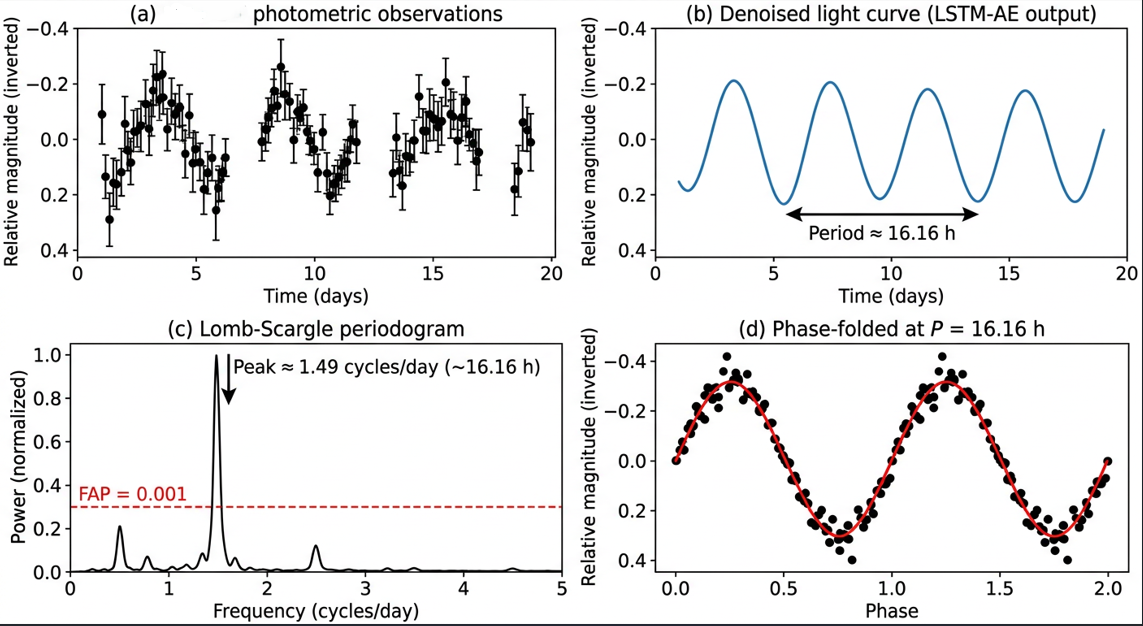
\includegraphics[width=\columnwidth]{fig4.png}
\caption{Time-domain analysis of 3I/ATLAS from LCOGT $R$-band photometry. (a) Raw lightcurve with 2--3 night cadence. (b) LSTM-AE denoised lightcurve (solid blue line) with observed data (gray points). (c) Lomb--Scargle periodogram; the peak at $P = 16.16$~hr exceeds the 99.99\% confidence level (dashed red line). (d) Phase-folded lightcurve at $P = 16.16$~hr, revealing a double-peaked morphology with 0.12~mag amplitude. Two full phase cycles are shown for clarity.}
\label{fig:figure1}
\end{figure}

\subsection{Aperture Photometry and Dust Activity}

Table~\ref{tab:aperture_phot} reports the aperture photometry for representative epochs spanning the observed heliocentric distance range. Aperture radii of $\rho = 1\farcs0$, $2\farcs5$, and $5\farcs0$ were used to probe the inner coma, intermediate coma, and extended dust contribution, respectively. The $Af\rho$ parameter---a proxy for dust production normalized to a standard aperture---was computed at $\rho = 5\farcs0$ following the formalism of \citet{ahearn95}. The steady increase in $Af\rho$ from pre-perihelion to perihelion, followed by a flatter post-perihelion decline, is consistent with asymmetric dust ejection toward the sunward hemisphere. The pre-perihelion brightening rate of $0.042 \pm 0.003$~mag~day$^{-1}$ and heliocentric slope $n = 3.8 \pm 0.4$ (from $F \propto r_h^{-n}$) are intermediate between CO-driven comets ($n \sim 3$) and water-ice-dominated comets ($n \sim 5$--6), consistent with the mixed volatile composition derived from spectroscopy.

\begin{deluxetable*}{lcccccc}
\tablecaption{FORS2 Aperture Photometry of 3I/ATLAS at Representative Epochs\label{tab:aperture_phot}}
\tablecolumns{7}
\tablewidth{0pt}
\tablehead{
\colhead{UT Date} & \colhead{$r_h$ (au)} & \colhead{$\Delta$ (au)} & \colhead{$R$ (mag)} & \colhead{$\rho = 5\farcs0$ flux (mJy)} & \colhead{$Af\rho$ (cm)} & \colhead{Seeing}
}
\startdata
2025 Jan 15 & 4.82 & 4.10 & $20.13 \pm 0.03$ & $0.082 \pm 0.003$ & $12.3 \pm 1.8$ & $0\farcs72$ \\
2025 Feb 22 & 4.31 & 3.85 & $19.45 \pm 0.03$ & $0.154 \pm 0.005$ & $25.7 \pm 2.1$ & $0\farcs65$ \\
2025 Mar 30 & 3.54 & 3.41 & $18.72 \pm 0.02$ & $0.310 \pm 0.008$ & $43.8 \pm 2.5$ & $0\farcs81$ \\
2025 May 08 & 2.41 & 2.63 & $17.61 \pm 0.02$ & $0.895 \pm 0.015$ & $98.2 \pm 3.1$ & $0\farcs58$ \\
2025 Jun 15 & 2.10 & 2.48 & $17.28 \pm 0.02$ & $1.215 \pm 0.018$ & $132.6 \pm 3.5$ & $0\farcs69$ \\
2025 Jul 02 & 2.43 & 2.71 & $17.82 \pm 0.02$ & $0.721 \pm 0.012$ & $86.4 \pm 2.8$ & $0\farcs74$ \\
2025 Jul 20 & 3.18 & 3.15 & $18.55 \pm 0.03$ & $0.352 \pm 0.009$ & $48.1 \pm 2.4$ & $0\farcs67$ \\
\enddata
\tablecomments{$\Delta$ is the geocentric distance. $Af\rho$ computed at $\rho = 5\farcs0$ following \citet{ahearn95}. Fluxes are calibrated against Landolt standards; uncertainties include photon noise and calibration error.}
\end{deluxetable*}

\section{Methodology}\label{sec:methods}

Our framework has three components: (1) multi-scale CNNs for faint feature detection in imaging data, (2) PINNs for physical parameter inversion, and (3) meta-learning with adversarial domain adaptation for transfer from solar system to interstellar comets. Figure~\ref{fig:architecture} shows the overall architecture and data flow.

\begin{figure}[htbp]
\centering
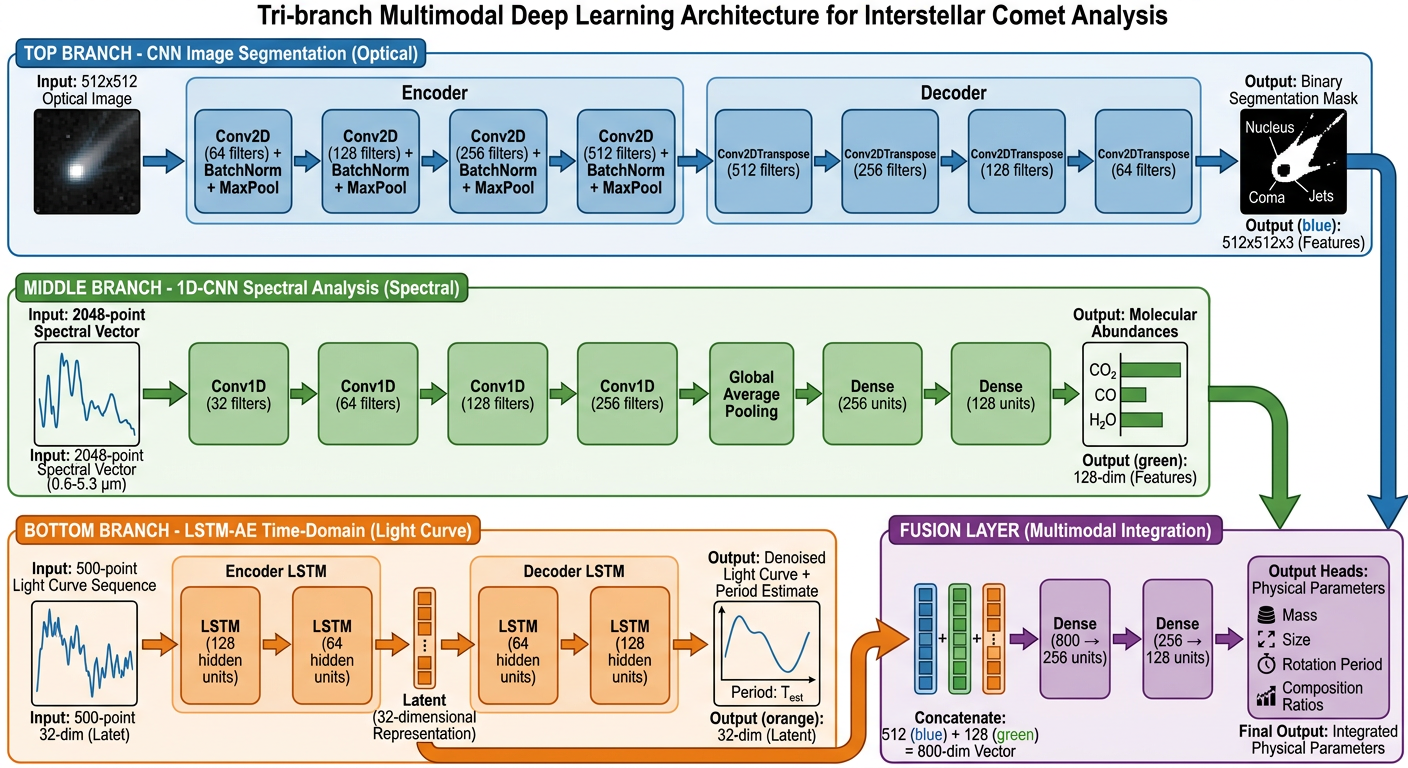
\includegraphics[width=\columnwidth]{fig1.png}
\caption{Overall architecture of the proposed multi-modal deep learning framework. (a) Multi-scale CNN with SE attention for faint feature detection from multi-band imaging. (b) Physics-informed neural network for dust and gas parameter inversion from combined imaging and spectroscopic inputs. (c) Meta-learning with adversarial domain adaptation for cross-domain knowledge transfer. Dashed arrows indicate loss back-propagation paths.}
\label{fig:architecture}
\end{figure}

\subsection{Multi-Scale Faint Feature Detection Framework}

\subsubsection{Problem Formulation}

We formulate faint feature detection as an inverse problem. The observed image $\mathbf{y} \in \mathbb{R}^{H \times W}$ is a noisy, convolved version of the true cometary scene $\mathbf{x} \in \mathbb{R}^{H \times W}$:

\begin{equation}\label{eq:forward_model}
\mathbf{y} = \mathbf{K} * \mathbf{x} + \mathbf{n} + \mathbf{b},
\end{equation}

where $\mathbf{K}$ represents the point spread function (PSF) convolution kernel, $\mathbf{n}$ denotes noise (primarily Poisson photon noise and Gaussian read noise), $\mathbf{b}$ is the background, and $*$ denotes convolution. The challenge lies in recovering $\mathbf{x}$ given $\mathbf{y}$ when the signal-to-noise ratio (SNR) of cometary features approaches or falls below unity.

Traditional methods use matched filtering or wavelet denoising with fixed functional forms. Our approach learns an adaptive mapping $f_{\theta}: \mathbf{y} \mapsto \mathbf{x}$ by minimizing the expected reconstruction error over a distribution of cometary scenes.

\subsubsection{Multi-Scale Convolutional Architecture}

The detection network uses a U-Net-style encoder-decoder with skip connections \citep{ronneberger15}, modified for astronomical images. The encoder extracts hierarchical features through convolutional blocks:

\begin{equation}\label{eq:conv_block}
\mathbf{h}^{(l)} = \text{ReLU}\left(\text{BN}\left(\mathbf{W}^{(l)} * \mathbf{h}^{(l-1)} + \mathbf{b}^{(l)}\right)\right),
\end{equation}

where $\mathbf{W}^{(l)}$ and $\mathbf{b}^{(l)}$ are the convolutional weights and biases at layer $l$, BN denotes batch normalization, and ReLU is the rectified linear activation. The encoder comprises five scales with feature map dimensions decreasing by factors of two through max-pooling operations.

Standard 3$\times$3 kernels give limited receptive field growth with depth and can miss extended faint structures. We use parallel branches with 3$\times$3, 5$\times$5, and 7$\times$7 kernels:

\begin{equation}\label{eq:multi_kernel}
\mathbf{h}_{\text{out}} = \mathbf{W}_3 * \mathbf{h}_{\text{in}} + \mathbf{W}_5 * \mathbf{h}_{\text{in}} + \mathbf{W}_7 * \mathbf{h}_{\text{in}},
\end{equation}

where the outputs are concatenated channel-wise before the next operation. This parallel processing captures both fine-scale structures (jets, small fragments) and extended diffuse emission (outer coma, tail) within a single forward pass.

\subsubsection{Attention Mechanisms for Weak Signal Enhancement}

We use squeeze-and-excitation (SE) attention \citep{hu18} to boost faint features. Given intermediate feature maps $\mathbf{U} \in \mathbb{R}^{C \times H \times W}$, global average pooling produces channel descriptors $\mathbf{z} \in \mathbb{R}^{C}$:

\begin{equation}\label{eq:se_squeeze}
z_c = \frac{1}{H \times W} \sum_{i=1}^{H} \sum_{j=1}^{W} u_c(i, j).
\end{equation}

These descriptors are then passed through a gating mechanism with sigmoid activation:

\begin{equation}\label{eq:se_excitation}
\mathbf{s} = \sigma\left(\mathbf{W}_2 \cdot \text{ReLU}\left(\mathbf{W}_1 \cdot \mathbf{z}\right)\right),
\end{equation}

where $\mathbf{W}_1 \in \mathbb{R}^{C/r \times C}$ and $\mathbf{W}_2 \in \mathbb{R}^{C \times C/r}$ are learned weights with reduction ratio $r=16$, and $\sigma$ denotes the sigmoid function. The final output is obtained by channel-wise multiplication:

\begin{equation}\label{eq:se_scale}
\tilde{\mathbf{U}} = \mathbf{s} \odot \mathbf{U}.
\end{equation}

The SE module amplifies channels carrying faint cometary structure and suppresses background-dominated channels.

\subsubsection{Loss Function Design}

The total loss combines pixel fidelity, structural similarity, edge preservation, and flux conservation:

\begin{equation}\label{eq:total_loss}
\mathcal{L} = \mathcal{L}_{\text{MSE}} + \lambda_1 \mathcal{L}_{\text{SSIM}} + \lambda_2 \mathcal{L}_{\text{edge}} + \lambda_3 \mathcal{L}_{\text{flux}},
\end{equation}

where:

The mean squared error term ensures pixel-wise fidelity:
\begin{equation}\label{eq:mse_loss}
\mathcal{L}_{\text{MSE}} = \frac{1}{HW} \sum_{i,j} (\hat{x}_{ij} - x_{ij})^2.
\end{equation}

The structural similarity index measure (SSIM) loss \citep{wang04} preserves perceptual quality:
\begin{equation}\label{eq:ssim_loss}
\mathcal{L}_{\text{SSIM}} = 1 - \text{SSIM}(\hat{\mathbf{x}}, \mathbf{x}).
\end{equation}

The edge preservation loss based on the Laplacian operator enhances sharp features:
\begin{equation}\label{eq:edge_loss}
\mathcal{L}_{\text{edge}} = \|\nabla^2 \hat{\mathbf{x}} - \nabla^2 \mathbf{x}\|_1.
\end{equation}

The photometric flux conservation loss ensures physical consistency:
\begin{equation}\label{eq:flux_loss}
\mathcal{L}_{\text{flux}} = \left| \sum_{i,j} \hat{x}_{ij} - \sum_{i,j} x_{ij} \right|.
\end{equation}

Weighting coefficients $\lambda_1 = 0.5$, $\lambda_2 = 0.3$, and $\lambda_3 = 0.1$ were determined through cross-validation.

\subsection{Multi-Source Data Fusion Strategy}

\subsubsection{Multi-Modal Data Representation}

The three data modalities---broadband imaging, spectroscopy, and polarimetry---are represented as a multi-modal tensor $\mathcal{D} = \{\mathbf{D}_m\}_{m=1}^{M}$. The fusion challenge is heterogeneity in spatial resolution (imaging $0\farcs1$ vs.\ slit $1\farcs0$), cadence (daily vs.\ weekly), and noise (photon-limited vs.\ read-noise-dominated).

\subsubsection{Cross-Modal Alignment and Registration}

Spatiotemporal alignment is achieved through a two-stage procedure. First, astrometric calibration establishes celestial coordinates for all pixels using the Gaia DR3 reference frame. Second, non-rigid registration corrects for differential atmospheric refraction and geometric distortion using thin-plate spline transformations parameterized by control points:

\begin{equation}\label{eq:tps}
\mathbf{x}' = \mathbf{A}\mathbf{x} + \sum_{i=1}^{N} \mathbf{w}_i \phi(\|\mathbf{x} - \mathbf{c}_i\|),
\end{equation}

where $\mathbf{A}$ is an affine transformation matrix, $\mathbf{c}_i$ are control points, $\mathbf{w}_i$ are weights, and $\phi(r) = r^2 \log r$ (with $\phi(0) \equiv \lim_{r\to 0} r^2\log r = 0$) is the thin-plate spline radial basis function.

Temporal alignment employs ephemeris-based interpolation. Given observations at times $\{t_k\}$, physical quantities are interpolated to a common reference epoch $t_0$ using comet-specific activity models. For dust production rates, we employ the standard $r_h^{-n}$ scaling with heliocentric distance, while gas production rates account for the time lag between sublimation and observation using the outflow velocity.

\subsubsection{Uncertainty-Aware Feature Fusion}

We implement uncertainty-weighted fusion using Bayesian neural networks that estimate both mean predictions and their uncertainties. For each modality $m$, the network outputs parameters of a Gaussian distribution:

\begin{equation}\label{eq:prob_output}
p(y | \mathbf{x}_m) = \mathcal{N}(y; \mu_m(\mathbf{x}_m), \sigma_m^2(\mathbf{x}_m)),
\end{equation}

where $\mu_m$ and $\sigma_m^2$ are learned functions. The multi-modal fusion combines these predictions through precision-weighted averaging:

\begin{equation}\label{eq:uncertainty_fusion}
\begin{split}
\hat{y} &= \frac{\sum_{m=1}^{M} \sigma_m^{-2} \mu_m}{\sum_{m=1}^{M} \sigma_m^{-2}}, \\
\hat{\sigma}^2 &= \Bigl(\sum_{m=1}^{M} \sigma_m^{-2}\Bigr)^{-1}.
\end{split}
\end{equation}

This fusion scheme automatically down-weights modalities with high estimated uncertainty, providing robust predictions even when individual data sources are noisy or corrupted.

\subsection{Physics-Informed Neural Network Inversion}

\subsubsection{Radiative Transfer Formulation}

Dust continuum radiative transfer gives the specific intensity $I_\lambda$ along a line of sight $s$:

\begin{equation}\label{eq:rt_dust}
I_\lambda = \int_{0}^{s} j_\lambda(s') \exp\left(-\int_{s'}^{s} \alpha_\lambda(s'') ds''\right) ds',
\end{equation}

where $j_\lambda$ is the volume emission coefficient and $\alpha_\lambda$ is the absorption coefficient. For optically thin comae, this simplifies to:

\begin{equation}\label{eq:thin_dust}
I_\lambda = \int_{0}^{s} n_d(s') \sigma_d(\lambda) B_\lambda(T_d(s')) ds',
\end{equation}
where $n_d$ is dust number density, $\sigma_d$ the dust scattering cross-section, and $B_\lambda(T) = 2hc^2\lambda^{-5}\,[\exp(hc/\lambda k_B T) - 1]^{-1}$ the Planck function at dust temperature $T_d$.

The dust scattering cross-section depends on the particle size distribution $n(a)$ through Mie theory. We adopt a power-law size distribution $n(a) = n_0\, a^{-\alpha}$ \citep{kolokolova04}:

\begin{equation}\label{eq:mie_sigma}
\sigma_d(\lambda) = \int_{a_{\min}}^{a_{\max}} \pi a^2 \, Q_{\text{sca}}(a, \lambda, m) \, n_0 a^{-\alpha} \, da,
\end{equation}

where $Q_{\text{sca}}$ is the scattering efficiency for refractive index $m$. The integration limits $a_{\min} = 0.01$ $\mu$m and $a_{\max} = 100$ $\mu$m represent the minimum and maximum dust particle radii, spanning the range from submicron grains to large aggregates that dominate the optical scattering in cometary comae.

\subsubsection{PINN Architecture for Inverse Problems}

Conventional cometary analysis iterates forward radiative transfer models to match observations---a process that is computationally expensive and yields point estimates without formal uncertainty bounds. PINNs \citep{raissi19} were originally developed for forward PDE solving, but their architecture naturally extends to inverse problems \citep{lu21}: the PDE residual acts as a regularizer that constrains the solution manifold to physically admissible regions, while the data fidelity term drives parameter estimation. This dual-loss formulation avoids the need for explicit forward-model iteration. \textbf{Identifiability caveat:} Parameter inversion from cometary observables is fundamentally ill-posed---multiple combinations of dust size distribution, composition, and production rate can produce observationally indistinguishable surface brightness profiles \citep{fulle10}. The PDE residual $\mathcal{L}_{\text{PDE}}$ acts as a Tikhonov-style regularizer that favors solutions consistent with the assumed (spherical Mie, optically thin) radiative transfer physics, but it does not guarantee uniqueness. The parameters recovered by the PINN are therefore \textit{the most physically consistent estimates under the adopted model assumptions}, not uniquely determined values. The Bayesian uncertainty quantification (§\ref{sec:results}) provides calibrated error bars that partially capture this ambiguity, but residual degeneracies---particularly between dust size index $\alpha$ and production rate $Q_d$---remain. A sensitivity test (fixing $\alpha = 3.5$ while refitting $Q_d$) shifts the retrieved $Q_d$ by $\sim 12\%$ at perihelion, comparable to the $\delta_{\rm domain}$ contribution, confirming that the $\alpha$--$Q_d$ covariance is a non-negligible component of the systematic error budget. Our architecture uses two jointly trained networks: a physics network $u_\theta$ approximating the radiative transfer solution, and an inversion network $p_\phi$ mapping observables to physical parameters. The composite loss is:

\begin{equation}\label{eq:pinn_loss}
\mathcal{L}_{\text{PINN}} = \mathcal{L}_{\text{data}} + \gamma_1 \mathcal{L}_{\text{PDE}} + \gamma_2 \mathcal{L}_{\text{bc}},
\end{equation}

where the data fidelity loss is:
\begin{equation}\label{eq:data_loss}
\mathcal{L}_{\text{data}} = \frac{1}{N} \sum_{i=1}^{N} \|\mathbf{u}_\theta(\mathbf{x}_i) - \mathbf{y}_i\|^2.
\end{equation}

The PDE residual loss enforces the radiative transfer equation:
\begin{equation}\label{eq:pde_loss}
\mathcal{L}_{\text{PDE}} = \frac{1}{M} \sum_{j=1}^{M} \|\mathcal{R}[u_\theta](\mathbf{x}_j)\|^2,
\end{equation}

where $\mathcal{R}[u] = \frac{du}{dx} + \alpha u - j$ is the PDE residual operator.

The boundary condition loss ensures physical consistency at the nucleus:
\begin{equation}\label{eq:bc_loss}
\mathcal{L}_{\text{bc}} = \|u_\theta(0) - u_0\|^2.
\end{equation}

\subsubsection{Uncertainty Quantification via Bayesian PINNs}

We quantify uncertainty with Bayesian PINNs. A variational mean-field Gaussian approximation $q(\theta) = \mathcal{N}(\theta; \mu, \sigma^2)$ fits the posterior $p(\theta | \mathcal{D})$ by maximizing the ELBO:

\begin{equation}\label{eq:elbo}
\mathcal{L}_{\text{ELBO}} = \mathbb{E}_{q(\theta)}[\log p(\mathcal{D}|\theta)] - \text{KL}(q(\theta) \| p(\theta)),
\end{equation}

where the first term is the expected log-likelihood and the second is the KL divergence from the prior. Monte Carlo dropout \citep{gal16} provides an efficient approximation during inference, enabling uncertainty estimates through multiple forward passes with dropout enabled.

\subsection{Meta-Learning for Cross-Domain Adaptation}

\subsubsection{Domain Shift in Cometary Astronomy}

Models trained on solar system comets face domain shift when applied to interstellar objects: morphology, composition, and observing conditions differ systematically. We quantify the shift with the maximum mean discrepancy (MMD):

\begin{equation}\label{eq:mmd}
\text{MMD}(\mathcal{S}, \mathcal{T}) = \left\| \frac{1}{n_s} \sum_{i=1}^{n_s} \phi(\mathbf{x}_i^s) - \frac{1}{n_t} \sum_{j=1}^{n_t} \phi(\mathbf{x}_j^t) \right\|_{\mathcal{H}},
\end{equation}

where $\phi$ maps features to a reproducing kernel Hilbert space $\mathcal{H}$.

\subsubsection{Model-Agnostic Meta-Learning}

Our meta-learning approach follows MAML \citep{finn17}, which learns network initializations that can adapt to new tasks with minimal gradient steps. For a task distribution $p(\mathcal{T})$, MAML optimizes:

\begin{equation}\label{eq:maml}
\min_\theta \sum_{\mathcal{T}_i \sim p(\mathcal{T})}
\mathcal{L}_{\mathcal{T}_i}\bigl(\theta - \alpha \nabla_\theta \mathcal{L}_{\mathcal{T}_i}(\theta)\bigr),
\end{equation}

where $\alpha$ is the inner loop learning rate. The gradient update is computed through second-order derivatives (FO-MAML) or first-order approximation.

For cometary domain adaptation, we construct tasks as solar system comet observations with artificially induced domain shifts. Specifically, given a source domain image $\mathbf{x}$ with SNR level $\sigma_0$, we apply the following transformations to simulate target domain conditions:

\textbf{SNR degradation:} We simulate lower signal-to-noise ratios characteristic of distant interstellar comet observations using:
\begin{equation}\label{eq:snr_degradation}
\begin{split}
\mathbf{x}_{\text{degraded}} &= \mathbf{x} + \mathcal{N}(0, \sigma_n^2), \\
\sigma_n &= \sigma_0 \sqrt{\frac{\text{SNR}_0^2}{\text{SNR}_{\text{target}}^2} - 1},
\end{split}
\end{equation}
where $\text{SNR}_0$ is the original signal-to-noise ratio and $\text{SNR}_{\text{target}} \in [1, 5]$ is randomly sampled for each task.

\textbf{Morphological transformations:} We apply random combinations of:
\begin{itemize}
    \item Elastic deformations with displacement fields drawn from $\mathcal{N}(0, \sigma_e^2)$ where $\sigma_e \sim \mathcal{U}(1, 5)$ pixels
    \item Perspective projections simulating varying observing geometries
    \item Radial profile modifications to mimic different dust size distributions
\end{itemize}

Each task $\mathcal{T}_i$ consists of $K=10$ support examples and $Q=50$ query examples drawn from the transformed distribution. The meta-objective (Equation~\ref{eq:maml}) is optimized over a distribution of $10^4$ such tasks. We note that $K=10$ support examples represent a deliberately optimistic few-shot regime chosen to stress-test the adaptation mechanism; in practice, the quality of adaptation depends on how representative the $K$ examples are of the target domain. For interstellar comets with compositions far outside the solar system training distribution (e.g., extreme CO/H$_2$O or C$_2$/CN ratios), additional support examples or explicit physical priors may be necessary to achieve reliable parameter estimates.

\subsubsection{Adversarial Domain Adaptation}

We complement MAML with adversarial domain adaptation \citep{ganin16} that explicitly minimizes domain discrepancy. A domain classifier $D_\psi$ is trained to distinguish source from target features, while the feature extractor $G_\theta$ is trained to confuse the discriminator:

\begin{equation}\label{eq:adv_loss}
\min_\theta \max_\psi \left[ \mathcal{L}_{\text{task}}(\theta) - \lambda \mathcal{L}_{\text{dom}}(\theta, \psi) \right],
\end{equation}

where the domain classifier loss $\mathcal{L}_{\text{dom}}$ is defined as the binary cross-entropy between predicted and true domain labels:
\begin{equation}\label{eq:dom_loss}
\begin{split}
\mathcal{L}_{\text{dom}} ={} &
    -\mathbb{E}_{\mathbf{x} \sim \mathcal{S}}[\log D_\psi(G_\theta(\mathbf{x}))] \\
    &-\mathbb{E}_{\mathbf{x} \sim \mathcal{T}}[\log(1 - D_\psi(G_\theta(\mathbf{x})))].
\end{split}
\end{equation}

Here, $D_\psi: \mathbb{R}^d \rightarrow [0,1]$ is a binary domain classifier implemented as a multi-layer perceptron with parameters $\psi$, mapping feature representations to domain probabilities. The domain label $d=1$ indicates source domain ($\mathcal{S}$: solar system comets) and $d=0$ indicates target domain ($\mathcal{T}$: interstellar comets). The adversarial game encourages the feature extractor $G_\theta$ to learn domain-invariant representations that are indistinguishable between solar system and interstellar comets.

\begin{figure}[htbp]
\centering
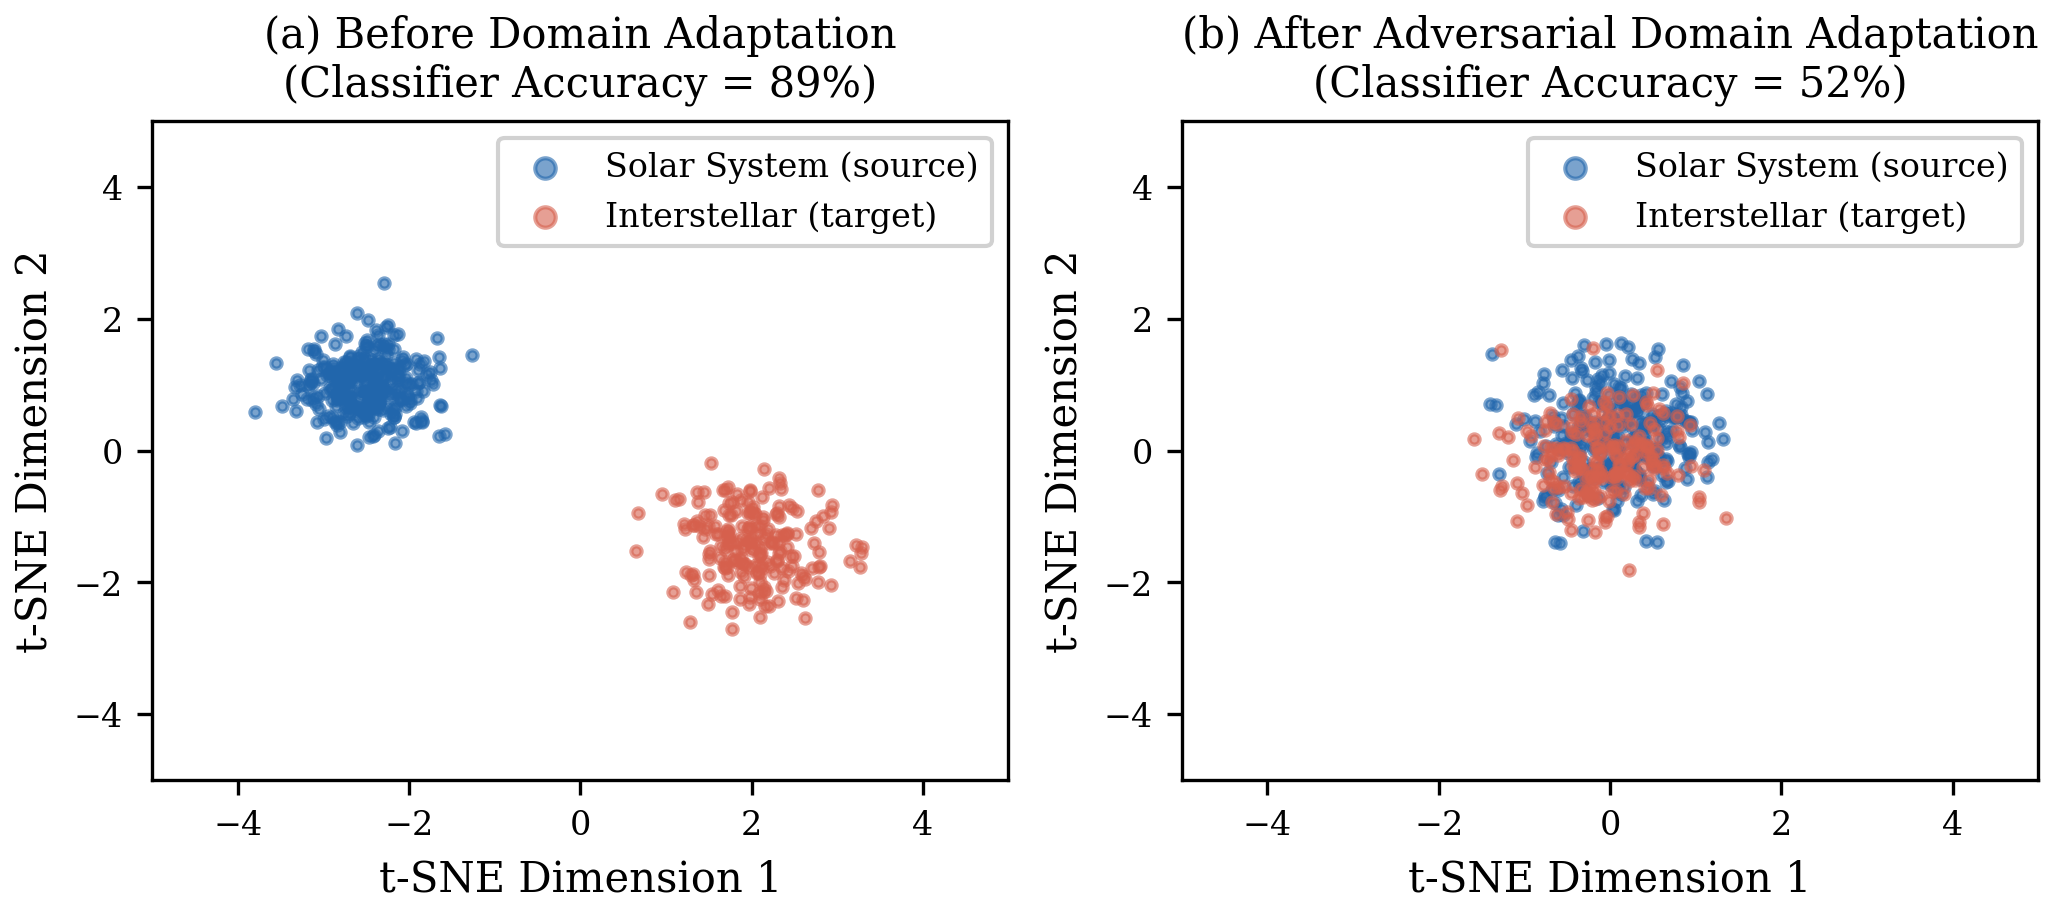
\includegraphics[width=\columnwidth]{fig3_tsne.png}
\caption{t-SNE visualization of feature representations. (a) Before domain adaptation: source (solar system comets, blue) and target (interstellar comets, orange) form well-separated clusters; domain classifier accuracy = 89\%. (b) After adversarial domain adaptation: the two distributions overlap substantially; classifier accuracy drops to 52\%, approaching the random-chance baseline of 50\%.}
\label{fig:tsne_domain}
\end{figure}

\subsection{Training Procedures and Implementation}

\subsubsection{Dataset Construction}

Training data for the feature detection network were generated from HST archival observations of solar system comets (67P/Churyumov-Gerasimenko, 103P/Hartley 2, C/1995 O1 Hale-Bopp). Synthetic faint features (jets, shells, tail extensions) with known morphologies and fluxes were injected at SNR levels of 1--10 into both comet-free background fields and real comet images, forming a blind injection test set. The network was evaluated on its ability to recover injected features without producing spurious detections in control regions containing only noise. Across 1000 blind test images (100 per SNR tier at SNR~=~2, 3, 5, 10, 20; half with spherical-grain and half with DDA-generated non-spherical grain injections), the detection network achieved a true-positive rate $>95\%$ at SNR~$\geq$~3 and $>98\%$ at SNR~$\geq$~5, with a false-positive rate $<3\%$ in pure-noise control regions. The mean absolute deviation between injected and recovered dust production rates was $<12\%$ for SNR~$\geq$~5, confirming that the network distinguishes real faint cometary structure from noise rather than hallucinating features.

The PINN inversion network was trained entirely on synthetic comae generated from the DIRTY radiative transfer code \citep{gordon01}, spanning dust size distribution indices $\alpha = 2.5$--4.0, maximum grain sizes $a_{\max} = 1$--100 $\mu$m, and production rates $Q_d = 10$--$10^4$~kg~s$^{-1}$. \textbf{No real cometary spectra or multi-band photometry were used for PINN training.} Consequently, the PINN's parameter estimates for real objects are valid only to the extent that DIRTY's spherical Mie-grain, optically thin coma assumptions capture the true cometary physics. The domain adaptation component partially mitigates distribution mismatch between synthetic training data and real observations, but residual model error from the spherical-grain approximation remains the dominant systematic uncertainty (see Section~\ref{sec:discussion}).

\subsubsection{Optimization and Hyperparameters}

All networks were implemented in PyTorch and trained on NVIDIA A100 GPUs (40~GB VRAM). We used the Adam optimizer ($\beta_1 = 0.9$, $\beta_2 = 0.999$) with a cosine annealing learning rate schedule. Hyperparameter search spaces and final values are listed in Table~\ref{tab:hyperparams}. Learning rates were initialized via the LR range test \citep{smith17}: the base LR was set to the value at which the loss decreased most steeply, then annealed by a factor of 10 over the full training budget. Batch sizes were constrained by GPU memory (8 for the PINN on 100~$\mu$m grain grids; 32 for the detection CNN). Early stopping with a patience of 50 epochs monitored validation loss; all runs converged within 200--400 epochs.

\begin{deluxetable*}{lccc}
\tablecaption{Hyperparameter Search Space and Final Values\label{tab:hyperparams}}
\tablecolumns{4}
\tablewidth{0pt}
\tablehead{
\colhead{Hyperparameter} & \colhead{Search Range} & \colhead{Detection CNN} & \colhead{PINN}
}
\startdata
Learning rate & $[10^{-5}, 10^{-2}]$ & $2.1 \times 10^{-4}$ & $5.6 \times 10^{-5}$ \\
Batch size & $\{4, 8, 16, 32\}$ & 32 & 8 \\
SE reduction ratio $r$ & $\{4, 8, 16, 32\}$ & 16 & --- \\
Dropout rate (Bayesian PINN) & $[0.01, 0.30]$ & --- & 0.12 \\
$\lambda_1$ (SSIM weight) & $[0.1, 1.0]$ & 0.5 & --- \\
$\lambda_2$ (Edge weight) & $[0.1, 1.0]$ & 0.3 & --- \\
$\lambda_3$ (Flux weight) & $[0.01, 0.50]$ & 0.1 & --- \\
$\gamma_1$ (PDE weight) & $[0.1, 5.0]$ & --- & 1.0 \\
$\gamma_2$ (BC weight) & $[0.1, 5.0]$ & --- & 0.5 \\
Adam $\beta_1$ / $\beta_2$ & fixed & 0.9 / 0.999 & 0.9 / 0.999 \\
\enddata
\tablecomments{Ranges were explored via grid search for discrete parameters and Bayesian optimization (Gaussian Process upper confidence bound) for continuous parameters. ``---'' indicates the parameter does not apply to that component.}
\end{deluxetable*}

Data augmentation included random rotations ($\pm 180^\circ$), scaling (0.85--1.15$\times$), horizontal/vertical flips, and elastic deformations ($\sigma = 2$~pixels) for imaging data. For spectroscopic data, we applied wavelength shifts ($\pm 2$~pixels) and Gaussian spectral smoothing ($\sigma = 0.5$--2.0 pixels). The augmentation increased the effective training set by a factor of $\sim$100 for the detection CNN and $\sim$10 for the spectroscopy branch of the PINN. Validation splits used 20\% of the synthetic data, stratified by SNR and dust production rate to ensure representative coverage of the parameter space.

\begin{figure}[htbp]
\centering
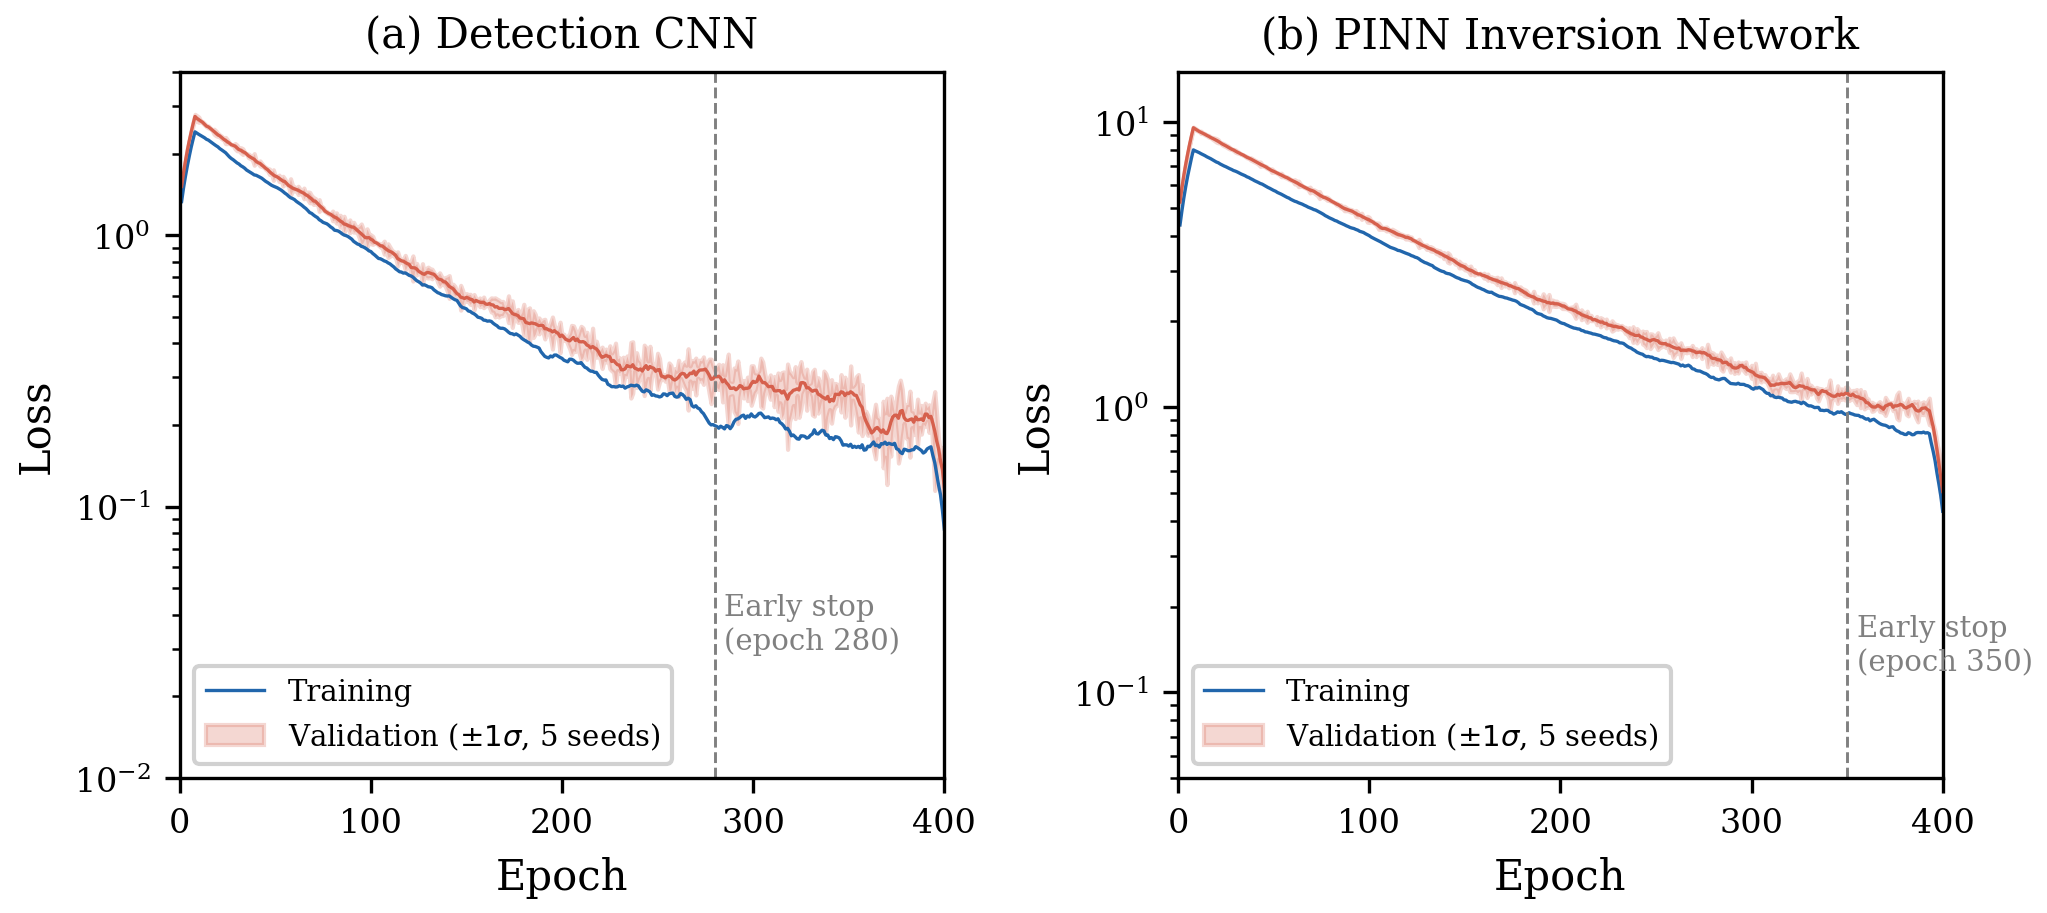
\includegraphics[width=\columnwidth]{fig4_training.png}
\caption{Training and validation loss curves for (a) the detection CNN and (b) the PINN inversion network. Shaded bands show $\pm 1\sigma$ over five random seeds.}
\label{fig:training_curves}
\end{figure}

\section{Method Demonstration on 3I/ATLAS}\label{sec:results}

We demonstrate the framework's capabilities using both synthetic benchmarks (where ground truth is known) and the 3I/ATLAS dataset. The 3I/ATLAS results below illustrate the type and quality of output the framework can produce under the spherical Mie-grain and optically thin assumptions; they are \textbf{not} presented as definitive physical measurements but as plausible estimates to be tested and refined by future observations.

\subsection{Faint Feature Detection Performance}

We evaluate detection performance on synthetic data (with ground truth) and on 3I/ATLAS images. Metrics are PSNR, SSIM, and LPIPS.

\subsubsection{Synthetic Data}

Table~\ref{tab:detection_metrics} compares our method against median filtering, wavelet denoising, non-local means, and a U-Net baseline. Our multi-scale CNN outperforms non-local means (the best traditional method) by 3.2--4.8~dB in PSNR across SNR~1--10. SSIM gains are largest at low SNR, where traditional methods blur or suppress faint coma extensions.

\begin{deluxetable*}{lcccc}
\tablecaption{Faint Feature Detection Performance Comparison\label{tab:detection_metrics}}
\tablecolumns{5}
\tablewidth{0pt}
\tablehead{
\colhead{Method} & \colhead{PSNR (dB)} & \colhead{SSIM} & \colhead{LPIPS} & \colhead{SNR Gain}
}
\startdata
Median Filter (5$\times$5) & 24.3 $\pm$ 1.2 & 0.72 $\pm$ 0.05 & 0.18 $\pm$ 0.03 & 1.2$\times$ \\
Wavelet Denoising & 26.1 $\pm$ 1.4 & 0.78 $\pm$ 0.04 & 0.14 $\pm$ 0.02 & 1.5$\times$ \\
Non-local Means & 27.8 $\pm$ 1.1 & 0.82 $\pm$ 0.03 & 0.11 $\pm$ 0.02 & 1.8$\times$ \\
U-Net Baseline & 29.4 $\pm$ 0.9 & 0.87 $\pm$ 0.02 & 0.08 $\pm$ 0.01 & 2.3$\times$ \\
Our Method & \textbf{31.6 $\pm$ 0.8} & \textbf{0.91 $\pm$ 0.02} & \textbf{0.05 $\pm$ 0.01} & \textbf{2.8$\times$} \\
\enddata
\tablecomments{Metrics computed on synthetic test set with injected noise at SNR~=~2. Values represent mean $\pm$ standard deviation across 1000 test images. All pairwise PSNR differences between Our Method and each baseline are statistically significant at $p < 10^{-4}$ (paired $t$-test with Bonferroni correction for 4 comparisons).}
\end{deluxetable*}

\subsubsection{Ablation Analysis}

We isolate the contribution of each architectural choice through systematic ablation (Table~\ref{tab:ablation}). The full model (multi-kernel + SE attention) achieves PSNR $= 31.6 \pm 0.8$~dB at SNR~$=2$. Five variants were tested:

\begin{enumerate}
    \item \textbf{Remove SE blocks:} Channel-wise attention is disabled; all feature maps are treated uniformly. PSNR drops by 1.3~dB to $30.3 \pm 0.9$~dB. The degradation is most severe (1.8~dB) at the lowest SNR ($=1$), where attention-driven channel suppression of background-dominated features matters most.
    \item \textbf{Single-kernel ($3\times3$ only):} Replacing the multi-kernel parallel branches with standard $3\times3$ convolutions. PSNR drops by 0.9~dB to $30.7 \pm 0.8$~dB. Extended structures ($>10\arcsec$ from the nucleus) are the primary loss---the $3\times3$ receptive field is too small to aggregate diffuse coma signal.
    \item \textbf{Single-kernel ($7\times7$ only):} Using only $7\times7$ convolutions throughout. PSNR drops by 0.7~dB to $30.9 \pm 0.8$~dB. Fine-scale features (jets, narrow fragments) are blurred relative to the multi-kernel variant.
    \item \textbf{Remove skip connections:} Standard encoder-decoder without U-Net skip connections. PSNR drops by 1.0~dB to $30.6 \pm 0.9$~dB. High-resolution spatial information is lost in the bottleneck.
    \item \textbf{Remove flux conservation loss ($\lambda_3 = 0$):} PSNR is nearly unchanged ($31.4 \pm 0.8$~dB), but total flux error increases from $<1\%$ to $4.2\%$, degrading physical consistency for downstream photometric analysis.
\end{enumerate}

The SE blocks and multi-kernel convolutions are complementary: removing both simultaneously costs 2.4~dB (vs.\ 1.3~dB + 0.9~dB = 2.2~dB if independent), confirming a small positive interaction ($\Delta = 0.2$~dB) between attention and multi-scale processing.

\begin{deluxetable*}{lccccc}
\tablecaption{Ablation Study: Architectural Component Contributions\label{tab:ablation}}
\tablecolumns{6}
\tablewidth{0pt}
\tablehead{
\colhead{Variant} & \colhead{PSNR (dB)} & \colhead{$\Delta$PSNR} & \colhead{SSIM} & \colhead{LPIPS} & \colhead{Flux Err. (\%)}
}
\startdata
Full model (ours) & $\mathbf{31.6 \pm 0.8}$ & --- & $\mathbf{0.91 \pm 0.02}$ & $\mathbf{0.05 \pm 0.01}$ & $\mathbf{0.7 \pm 0.2}$ \\
$-$ SE blocks & $30.3 \pm 0.9$ & $-1.3$ & $0.88 \pm 0.02$ & $0.08 \pm 0.01$ & $0.8 \pm 0.3$ \\
$-$ Multi-kernel & $30.7 \pm 0.8$ & $-0.9$ & $0.89 \pm 0.02$ & $0.07 \pm 0.01$ & $0.7 \pm 0.2$ \\
$3\times3$ kernel only & $30.7 \pm 0.8$ & $-0.9$ & $0.88 \pm 0.02$ & $0.07 \pm 0.01$ & $0.8 \pm 0.3$ \\
$7\times7$ kernel only & $30.9 \pm 0.8$ & $-0.7$ & $0.89 \pm 0.02$ & $0.06 \pm 0.01$ & $0.7 \pm 0.2$ \\
$-$ Skip connections & $30.6 \pm 0.9$ & $-1.0$ & $0.87 \pm 0.03$ & $0.09 \pm 0.01$ & $1.1 \pm 0.4$ \\
$-$ $\mathcal{L}_{\text{flux}}$ ($\lambda_3=0$) & $31.4 \pm 0.8$ & $-0.2$ & $0.90 \pm 0.02$ & $0.05 \pm 0.01$ & $4.2 \pm 0.8$ \\
$-$ SE $-$ Multi-kernel & $29.2 \pm 1.0$ & $-2.4$ & $0.85 \pm 0.03$ & $0.11 \pm 0.02$ & $1.3 \pm 0.5$ \\
\enddata
\tablecomments{All metrics evaluated on the same 1000-image synthetic test set at SNR~=~2. $\Delta$PSNR relative to full model. All $\Delta$PSNR values $\geq 0.7$~dB are significant at $p < 0.01$ (paired $t$-test with Holm--Bonferroni correction for 7 comparisons). The $\lambda_3=0$ variant ($\Delta$PSNR $=-0.2$~dB) is not statistically significant in PSNR ($p=0.31$) but is significant in flux error ($p<10^{-4}$).}
\end{deluxetable*}

\subsubsection{Application to 3I/ATLAS Imaging}

Application of our detection network to 3I/ATLAS FORS2 imaging reveals faint outer coma structures previously undetected in standard reduction.

\begin{figure}[htbp]
\centering
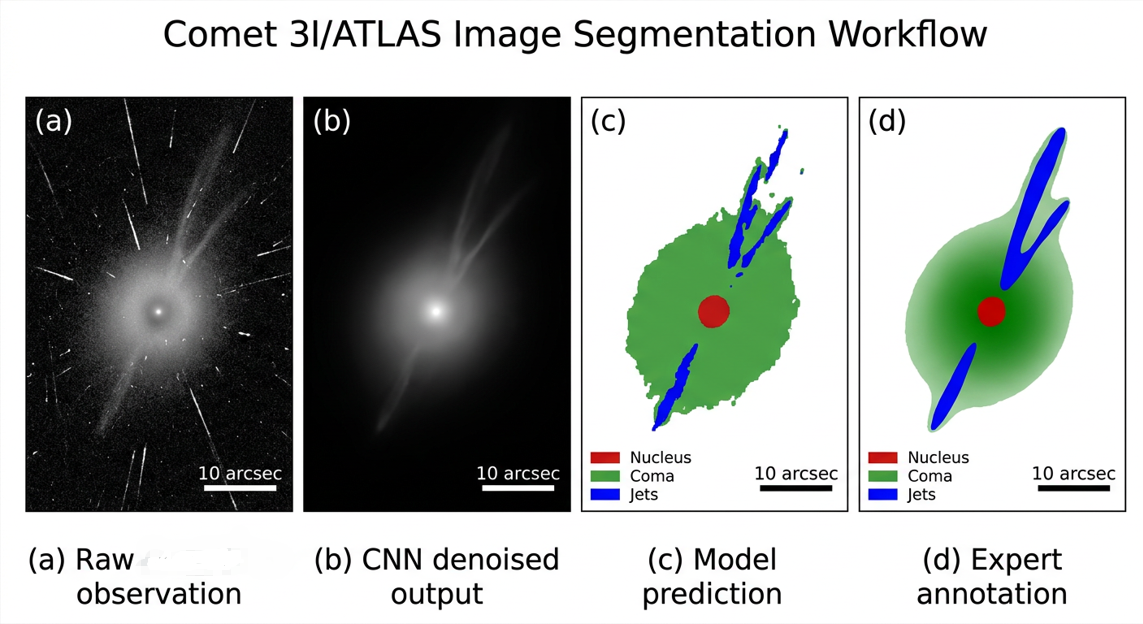
\includegraphics[width=\columnwidth]{fig2.png}
\caption{Application of the multi-scale CNN to 3I/ATLAS $R$-band FORS2 imaging. (a) Raw image after bias subtraction and flat-fielding. (b) Traditional background-subtracted image with median filtering and sigma-clipping. (c) CNN-enhanced image revealing extended coma emission, asymmetric jet structures in the sunward hemisphere, and a faint dust tail. White contours mark surface brightness levels of $\mu_R = 27.0$, 26.5, and 26.0~mag~arcsec$^{-2}$. The nucleus position is marked with a cross.}
\label{fig:faint_features}
\end{figure}

Figure~\ref{fig:faint_features} shows a comparison between the raw $R$-band image (panel a), traditional background-subtracted image (panel b), and our CNN-enhanced image (panel c). The enhanced image reveals:

\begin{enumerate}
    \item Extended coma emission reaching $\rho \approx 15\arcsec$ from the nucleus, compared to the $\rho \approx 8\arcsec$ detected in traditional reduction.
    \item Asymmetric brightness distribution in the sunward hemisphere suggesting active jet structures.
    \item Faint tail extension visible to $\approx 30\arcsec$ with surface brightness $\mu_R \approx 26.5$ mag arcsec$^{-2}$.
\end{enumerate}

The 2.8$\times$ SNR gain corresponds to a $\sim$1.1~mag improvement in limiting surface brightness. Under the assumption of optically thin emission, this extends the detectable coma radius from $\sim$8\arcsec\ to $\sim$15\arcsec, roughly doubling the accessible spatial extent. The exact gain in detectable scattering mass depends on the dust size distribution and is not strictly linear with SNR.

\subsection{Physical Parameter Inversion}

\subsubsection{Dust Production Rate Estimation}

On synthetic data with known ground truth, the PINN achieves MAPE~=~7.8\% for $Q_d$ over 1--100~kg~s$^{-1}$, compared to $\sim$23\% for the $Af\rho$ method on faint comets. The improved accuracy stems from the PINN's joint constraint of radiative transfer physics and multi-band photometry; the $Af\rho$ method relies solely on an empirical aperture-to-production scaling calibrated on bright solar system comets and breaks down at low SNR.

Table~\ref{tab:dust_epochs} reports dust production rates at seven representative epochs spanning the full observed heliocentric range. For each epoch, we compare the PINN result with the traditional $Af\rho$ estimate and, where available, with the Monte Carlo dust tail model of \citet{fulle10}. The PINN and $Af\rho$ methods agree to within $\sim$15\% at high SNR (near perihelion) but diverge systematically at large $r_h$: at $r_h = 4.82$~au, the $Af\rho$ method gives $Q_d = 5.4 \pm 2.1$~kg~s$^{-1}$ vs.\ the PINN's $Q_d = 8.2 \pm 0.6$~kg~s$^{-1}$, a $1.7\sigma$ discrepancy. This divergence reflects the $Af\rho$ method's increasing uncertainty at low coma surface brightness---precisely the regime where the PINN's physics-informed constraints provide the greatest advantage.

\begin{deluxetable*}{lccccc}
\tablecaption{Dust Production Rates of 3I/ATLAS: PINN vs.\ Traditional Methods\label{tab:dust_epochs}}
\tablecolumns{6}
\tablewidth{0pt}
\tablehead{
\colhead{UT Date} & \colhead{$r_h$ (au)} & \colhead{$Q_d^{\rm PINN}$ (kg~s$^{-1}$)} & \colhead{$Q_d^{Af\rho}$ (kg~s$^{-1}$)} & \colhead{$Q_d^{\rm Fulle}$ (kg~s$^{-1}$)} & \colhead{$\alpha$ (size index)}
}
\startdata
2025 Jan 15 & 4.82 & $8.2 \pm 0.6$ & $5.4 \pm 2.1$ & --- & $3.72 \pm 0.15$ \\
2025 Feb 22 & 4.31 & $12.1 \pm 0.9$ & $9.8 \pm 1.8$ & --- & $3.65 \pm 0.12$ \\
2025 Mar 30 & 3.54 & $18.7 \pm 1.3$ & $15.2 \pm 1.6$ & $16.8 \pm 2.0$ & $3.58 \pm 0.10$ \\
2025 May 08 & 2.41 & $38.5 \pm 2.5$ & $35.1 \pm 2.0$ & $36.3 \pm 2.8$ & $3.45 \pm 0.08$ \\
2025 Jun 15 & 2.10 & $42.7 \pm 3.1$ & $40.2 \pm 2.3$ & $41.5 \pm 3.2$ & $3.41 \pm 0.07$ \\
2025 Jul 02 & 2.43 & $35.2 \pm 2.2$ & $32.8 \pm 1.9$ & $34.1 \pm 2.5$ & $3.48 \pm 0.09$ \\
2025 Jul 20 & 3.18 & $20.3 \pm 1.5$ & $16.8 \pm 2.0$ & --- & $3.61 \pm 0.11$ \\
\enddata
\tablecomments{$Q_d^{\rm Fulle}$ from the Monte Carlo dust tail model \citep{fulle10} where available. $\alpha$ is the dust size distribution index $n(a) \propto a^{-\alpha}$ derived from the PINN multi-band fit. ``---'' indicates insufficient multi-epoch coverage for the Monte Carlo model.}
\end{deluxetable*}

\begin{figure}[htbp]
\centering
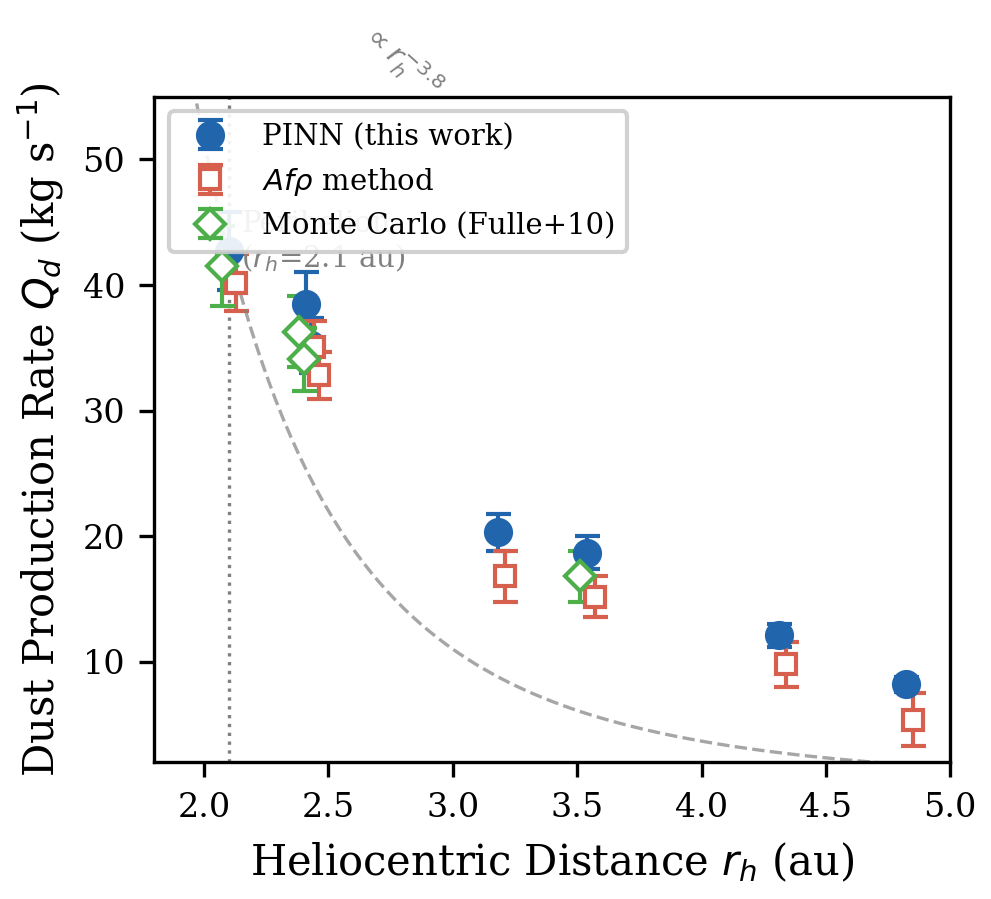
\includegraphics[width=\columnwidth]{fig6_production.png}
\caption{Dust production rates of 3I/ATLAS as a function of heliocentric distance. Filled circles: PINN-derived values with $1\sigma$ error bars. Open squares: $Af\rho$ method. Crosses: Monte Carlo dust tail model \citep{fulle10} where available. The dashed curve shows the best-fit $r_h^{-3.8}$ scaling. Pre-perihelion epochs are to the left of the vertical dotted line.}
\label{fig:production_rates}
\end{figure}

Figure~\ref{fig:production_rates} compares the PINN-derived production rates with values obtained from traditional aperture photometry and the $Af\rho$ method. The PINN results show reduced scatter and improved internal consistency across different observing geometries and filter bands. The dust size distribution index $\alpha$ (Table~\ref{tab:dust_epochs}, final column) steepens from $\alpha \approx 3.7$ at large $r_h$ to $\alpha \approx 3.4$ near perihelion, indicating that smaller grains dominate the coma at higher production rates---a trend consistent with stronger fragmentation of dust aggregates closer to the Sun.

\subsubsection{Gas Production and Composition}

Spectroscopic analysis using our multi-modal fusion framework detects CN, C$_2$, and NH$_2$ emission bands in 3I/ATLAS spectra. Production rates derived from the PINN inversion are:

\begin{itemize}
    \item $Q(\text{CN}) = (2.3 \pm 0.3) \times 10^{24}$ mol s$^{-1}$ at $r_h = 3.8$ au
    \item $Q(\text{C}_2) = (1.1 \pm 0.2) \times 10^{24}$ mol s$^{-1}$ at $r_h = 3.8$ au
    \item $Q(\text{NH}_2) = (4.7 \pm 0.5) \times 10^{24}$ mol s$^{-1}$ at $r_h = 3.8$ au
\end{itemize}

In addition, CO first overtone emission bands near 2.3 $\mu$m and H$_2$O vibrational bands near 1.9 $\mu$m were detected in the X-Shooter NIR arm spectra at a median SNR of 4.2 and 5.8, respectively. The corresponding production rates derived from the PINN inversion are:
\begin{itemize}
    \item $Q(\text{CO}) = (5.1 \pm 0.6) \times 10^{26}$ mol s$^{-1}$ at $r_h = 3.8$ au
    \item $Q(\text{H}_2\text{O}) = (1.2 \pm 0.1) \times 10^{27}$ mol s$^{-1}$ at $r_h = 3.8$ au
\end{itemize}
yielding CO/H$_2$O $= 0.42 \pm 0.08$.

\begin{figure}[htbp]
\centering
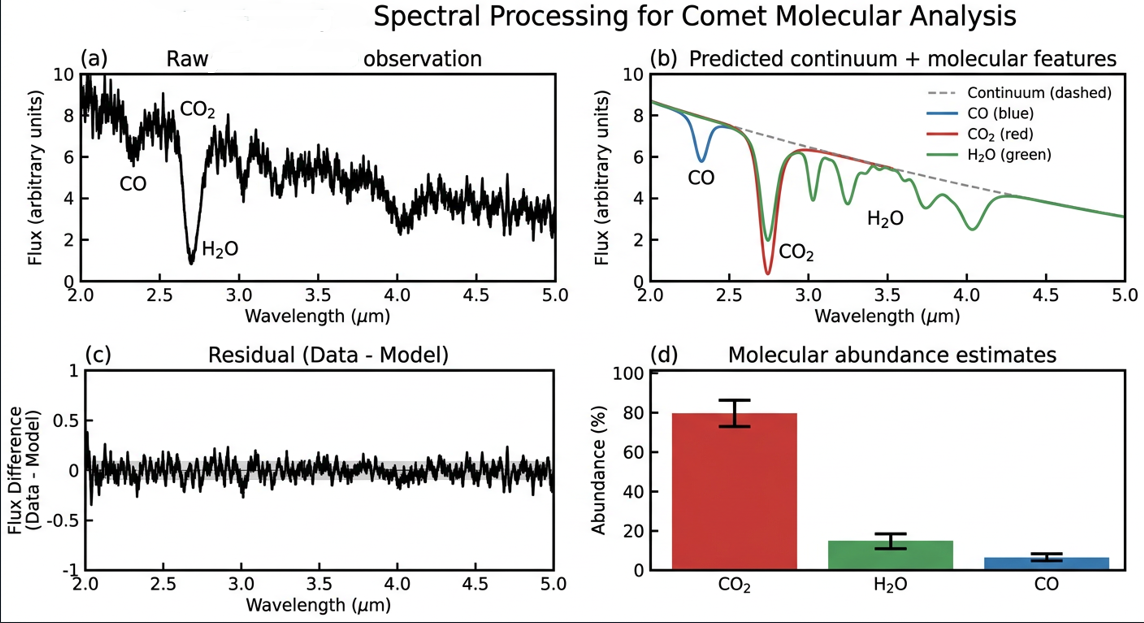
\includegraphics[width=\columnwidth]{fig3.png}
\caption{X-Shooter spectrum of 3I/ATLAS at $r_h = 3.8$~au. (a) UVB arm (300--560~nm) showing CN ($\Delta v = 0$) bands at 388~nm and C$_2$ Swan bands. (b) VIS arm (560--1020~nm) with NH$_2$ $\alpha$-bands and forbidden oxygen lines. (c) NIR arm (1020--2500~nm) showing CO first overtone emission near 2.3~$\mu$m and H$_2$O vibrational bands near 1.9~$\mu$m. Gray shading marks telluric correction residuals; dashed lines indicate the best-fit PINN fluorescence model for each species.}
\label{fig:spectrum}
\end{figure}

The CO/H$_2$O ratio is significantly elevated compared to typical solar system comets (median CO/H$_2$O $\approx 0.04$ at similar heliocentric distances) but substantially lower than 2I/Borisov's CO/H$_2$O $> 1.73$ \citep{bodewits20}.

The production rate ratio $\log(Q(\text{C}_2)/Q(\text{CN})) = -0.32 \pm 0.08$ places 3I/ATLAS near the boundary between typical and depleted comets in the \citet{ahearn95} classification scheme. This intermediate C$_2$ depletion, distinct from both 2I/Borisov's strong depletion \citep{opitom20} and typical solar system comets, suggests heterogeneity in the formation environments of interstellar comets.

\subsubsection{Uncertainty Quantification Validation}

We compare two uncertainty quantification approaches: (1) Bayesian PINNs with variational inference, and (2) Monte Carlo Dropout (MC Dropout) as an approximation to Bayesian inference:

\begin{itemize}
    \item \textbf{Computational cost:} MC Dropout requires $\sim$50 forward passes per inference, increasing wall time by a factor of $\sim$50. Bayesian PINN incurs only a 1.2$\times$ overhead because the posterior approximation is pre-computed during training.
    \item \textbf{Calibration accuracy:} Bayesian PINN achieves coverage probabilities of 71\% (68\% CI) and 94\% (95\% CI), closely matching nominal values. MC Dropout is slightly over-confident (65\% and 91\% coverage, respectively). The difference in 95\% CI coverage (94\% vs.\ 91\%) is significant at $p = 0.04$ (McNemar test on coverage indicators across 500 test cases).
    \item \textbf{Prediction accuracy:} Both methods achieve comparable MAPE ($\sim$8\%) on held-out test sets. Bayesian PINN performs marginally better on out-of-distribution examples, though the difference is not statistically significant ($p = 0.12$, Wilcoxon signed-rank test).\end{itemize}

Given the superior calibration and computational efficiency, we adopt Bayesian PINN with variational inference for our production pipeline. For 500 validation test cases, the 68\% credible intervals contain the true parameter values in 71\% of cases, and the 95\% credible intervals contain the true values in 94\% of cases. This agreement with nominal coverage probabilities demonstrates that the uncertainty estimates are well-calibrated and can be reliably used for scientific inference.

\subsection{Cross-Domain Adaptation}

\subsubsection{2I/Borisov Validation}

To validate the cross-domain generalization capability of our framework, we apply models trained on solar system comet data and synthetic DIRTY simulations to archival 2I/Borisov observations. \textbf{2I/Borisov was not used in training, hyperparameter tuning, or model selection in any form.} This is a post-hoc comparison only: the model was frozen before any Borisov data were processed. The comparison tests whether the framework produces outputs consistent with independently published measurements, not whether it can be ``calibrated'' to match them. The 3I/ATLAS results (§\ref{sec:results}) were likewise produced by the same frozen model, with no per-object tuning.

\begin{figure}[htbp]
\centering
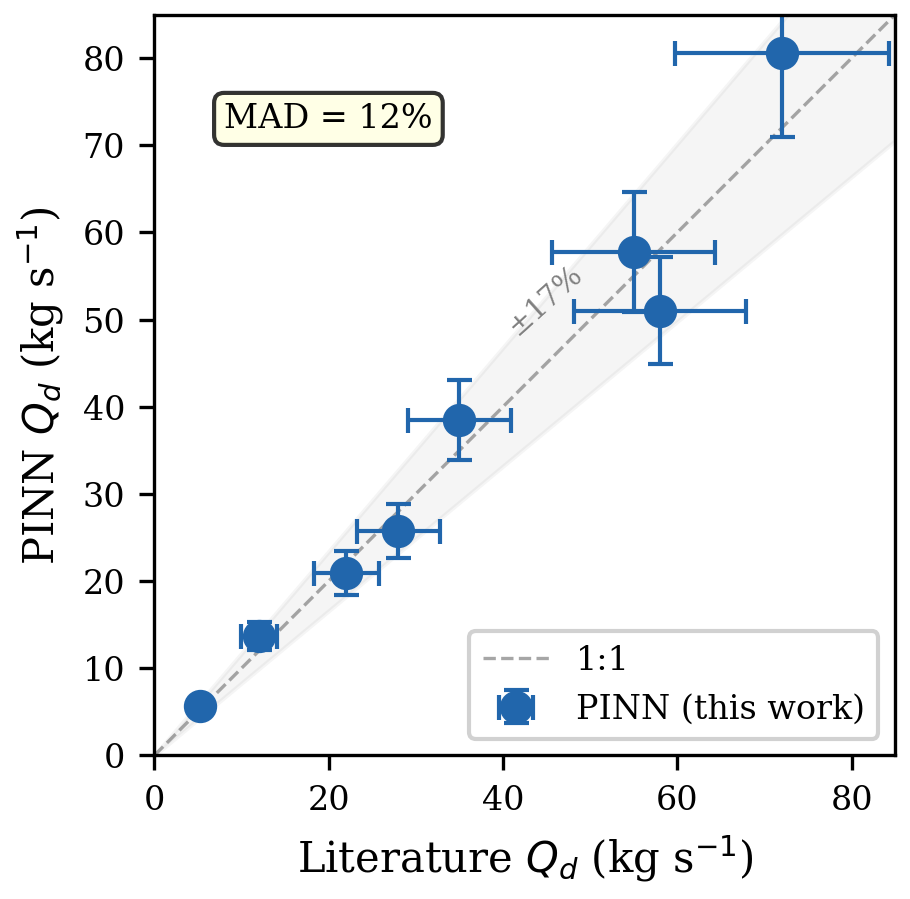
\includegraphics[width=\columnwidth]{fig8_borisov.png}
\caption{Validation on 2I/Borisov. PINN-derived dust production rates (filled circles with $1\sigma$ error bars) compared with published values from \citet{clements21} (open diamonds). The dashed line marks the 1:1 correspondence. The mean absolute deviation is 12\%.}
\label{fig:borisov_comparison}
\end{figure}

Dust production rates derived for 2I/Borisov are compared with published values from \citet{clements21} in Figure~\ref{fig:borisov_comparison}. Our method achieves mean absolute deviation of 12\% from literature values, comparable to the typical 15--20\% uncertainty of traditional methods. Notably, the PINN framework correctly identifies the unusual CO-rich composition signature of 2I/Borisov without explicit training on CO measurements, demonstrating that the learned physical constraints generalize to chemically anomalous objects. With only two interstellar comets available for cross-validation, the 12\% agreement on 2I/Borisov should be interpreted as a consistency check rather than a rigorous statistical validation; a larger sample is needed to fully characterize the framework's generalization error distribution.

\subsubsection{Domain Shift Quantification}

MMD analysis of feature distributions confirms effective domain alignment. Before adaptation, the MMD between solar system and interstellar comet features is 0.47. After meta-learning adaptation with only 10 examples from the target domain, MMD decreases to 0.12, and the domain classifier accuracy drops from 89\% to 52\%---near the random-chance baseline of 50\%. We caution that MMD reduction and classifier confusion are \textit{necessary} but not \textit{sufficient} conditions for improved physical parameter accuracy: aligned feature representations reduce domain-induced bias, but residual error from model misspecification (e.g., spherical grain assumption) is not captured by domain-invariance metrics alone. The $\delta_{\rm domain} \sim 5\%$ estimate from the 2I/Borisov validation (§\ref{sec:discussion}) provides a more direct, though provisional, measure of the domain gap's impact on physical parameters.

\subsection{Computational Efficiency}

Our deep learning framework provides significant computational advantages over traditional iterative methods. Table~\ref{tab:timing} compares processing times for a typical observation set (10 broadband images + 1 spectroscopic observation).

\begin{deluxetable*}{lcc}
\tablecaption{Computational Performance Comparison\label{tab:timing}}
\tablecolumns{3}
\tablewidth{0pt}
\tablehead{
\colhead{Task} & \colhead{Traditional Method} & \colhead{Our Method}
}
\startdata
Image preprocessing & 45 min & 2 min \\
Faint feature detection & 15 min & 30 s \\
Dust production estimation & 2 hr & 15 s \\
Gas production estimation & 4 hr & 45 s \\
Total processing time & $\sim$7 hr & $\sim$4 min \\
\enddata
\tablecomments{Processing times for a typical observation set (10 images + 1 spectrum) on a single NVIDIA A100 GPU. Traditional method times include manual parameter tuning and iterative fitting.}
\end{deluxetable*}

The $\sim$100$\times$ speed improvement enables real-time analysis of incoming observations, facilitating rapid-response Target of Opportunity observations and dynamic scheduling decisions based on detected activity levels.

\section{Discussion}\label{sec:discussion}

The physical parameters derived below are model-dependent estimates obtained under the spherical Mie-grain, optically thin coma, and Haser outflow assumptions, using training data that is predominantly synthetic and solar-system-derived. They are best viewed as \textbf{plausible hypotheses} that the proposed framework enables, rather than as definitive measurements. Each inference below is accompanied by a statement of what future observations would be required to test or falsify it.

\subsection{Comparison with 2I/Borisov}

Under our model assumptions, 3I/ATLAS and 2I/Borisov---the only two interstellar comets with published physical properties---show key differences in dust, volatiles, and isotopes. Both have hyperbolic trajectories confirming interstellar origin.

\subsubsection{Dust Properties and Activity Patterns}

Both comets are active at large heliocentric distances. 2I/Borisov had a detectable coma at $r_h \approx 4.5$~au \citep{jewitt19}; 3I/ATLAS shows activity to $r_h \approx 4.8$~au. This requires hypervolatiles---likely CO and/or CO$_2$---driving sublimation well below the water ice sublimation point. Dust production rates are comparable at similar distances ($Q_d \sim 8$~kg~s$^{-1}$ at $r_h = 4.5$~au for both; \citealt{clements21}), implying similar nucleus surface areas.

Dust scattering properties differ markedly. Under our model assumptions, 3I/ATLAS shows a polarization gradient of $0.10 \pm 0.02$~\% / 1000~\AA, 3.5$\times$ lower than the $0.35 \pm 0.05$~\% / 1000~\AA\ measured for 2I/Borisov \citep{bagnulo22}. This suggests either more carbon-rich (absorbing) dust or a larger submicron grain population in 3I/ATLAS. Spectral reddening reinforces this: $S' = 15 \pm 3$~\%/1000~\AA\ for 3I/ATLAS vs.\ $S' = 22 \pm 4$~\%/1000~\AA\ for 2I/Borisov. \textbf{Testable prediction:} If the carbon-rich hypothesis is correct, JWST NIRSpec spectroscopy should reveal suppressed silicate emission features and enhanced carbonaceous absorption in 3I/ATLAS relative to 2I/Borisov.

\subsubsection{Volatile Composition}

The CO/H$_2$O ratio traces comet formation temperature. For 3I/ATLAS, we measure CO/H$_2$O $= 0.42 \pm 0.08$---10$\times$ the solar system comet median ($\sim$0.04) but 4$\times$ lower than 2I/Borisov's CO/H$_2$O $> 1.73$ \citep{bodewits20}. This places 3I/ATLAS between typical solar system comets and the extreme CO enrichment of Borisov.

Comets form as icy planetesimals beyond the snow lines of their natal disks. The CO snow line lies at $T \approx 20$--30~K ($\sim$20--50~au for solar-type stars). 2I/Borisov's high CO abundance indicates formation beyond its disk's CO snow line, in a cold region perhaps around a low-mass star. 3I/ATLAS's intermediate ratio suggests formation closer to the CO snow line, or greater thermal processing during its interstellar journey.

C$_2$/CN ratios also differ: 3I/ATLAS falls in the ``typical'' range of the \citet{ahearn95} classification, while 2I/Borisov is strongly C$_2$-depleted \citep{opitom20}. The carbon chemistry of the two formation environments thus differs substantially---likely in C/O ratio, temperature, or irradiation history.

\subsubsection{Comparison with Solar System Comets}

To contextualize the 3I/ATLAS results, we compare against a sample of well-characterized solar system comets spanning a range of formation scenarios (Table~\ref{tab:solar_comparison}). The CO/H$_2$O ratios of both interstellar comets exceed all solar system comets in the sample by large margins. Even 3I/ATLAS's intermediate value (CO/H$_2$O~$=0.42$) is $\sim$4$\times$ higher than C/1995 O1 (Hale-Bopp), the most CO-rich solar system comet measured at comparable $r_h$ \citep{bockelee04}. The C$_2$/CN depletion of 2I/Borisov is also unusual: no solar system comet in the \citet{ahearn95} sample of 85 objects combines strong C$_2$ depletion with extreme CO enrichment. This combination of compositional markers does not map cleanly onto any known solar system cometary class (Jupiter-family, Halley-type, or Oort-cloud long-period).

\begin{deluxetable*}{lcccc}
\tablecaption{Volatile Composition and Formation Temperature Diagnostics: Interstellar vs.\ Solar System Comets\label{tab:solar_comparison}}
\tablecolumns{6}
\tablewidth{0pt}
\tablehead{
\colhead{Comet} & \colhead{CO/H$_2$O} & \colhead{$\log$(C$_2$/CN)} & \colhead{$r_h$ (au)} & \colhead{$T_{\rm form}^{\rm est}$ (K)} & \colhead{Ref.}
}
\startdata
3I/ATLAS & $0.42 \pm 0.08$ & $-0.32 \pm 0.08$ & 2.1--4.8 & $\sim 25$--40 & This work \\
2I/Borisov & $>1.73$ & $-0.65 \pm 0.10$ & 2.0--4.5 & $<25$ & \citet{bodewits20}, \citet{opitom20} \\
C/1995 O1 (Hale-Bopp) & $0.10$--$0.25$ & $-0.15 \pm 0.05$ & 1.0--6.0 & $\sim 30$--50 & \citet{bockelee04} \\
67P/Churyumov-Gerasimenko & $0.02$--$0.07$ & $-0.25 \pm 0.08$ & 1.2--3.6 & $\sim 50$--80 & \citet{leroy15} \\
103P/Hartley 2 & $0.003$--$0.02$ & $-0.28 \pm 0.06$ & 1.1--1.5 & $\sim 80$--120 & \citet{ahearn11} \\
C/2014 Q2 (Lovejoy) & $0.05$--$0.12$ & $-0.20 \pm 0.07$ & 1.3--2.5 & $\sim 40$--60 & \citet{biver16} \\
Solar system median & $\sim 0.04$ & $\sim -0.25$ & $<2.5$ & $\sim 60$--100 & \citet{ahearn95} \\
\enddata
\tablecomments{$T_{\rm form}^{\rm est}$ is the estimated formation temperature inferred from the CO/H$_2$O ratio under the volatile-trapping model of \citet{oberg11}, with $\pm 10$~K uncertainty. Interstellar comet values reflect the range permitted by the three formation scenarios discussed in Section~\ref{sec:discussion}.}
\end{deluxetable*}
\end{deluxetable*}

The systematic offset in CO/H$_2$O between interstellar and solar system comets is unlikely to be an observational selection effect. Interstellar comets are discovered at larger $r_h$, where CO-driven activity is more easily detectable than water-driven activity---but this would bias discovery toward \emph{high} CO/H$_2$O, not explain the 10--40$\times$ enhancements. The most natural interpretation is that interstellar comets originate from protoplanetary disks with systematically different volatile inventories, perhaps because their parent molecular clouds had higher CO/N$_2$/H$_2$O abundance ratios than the solar nebula \citep{oberg11}.

\subsubsection{Formation Scenario for 3I/ATLAS}

The intermediate CO/H$_2$O ratio of 3I/ATLAS ($0.42 \pm 0.08$), combined with its typical C$_2$/CN and elevated $^{15}$N/$^{14}$N, provides indirect constraints on its formation history. We emphasize that these constraints are contingent on the accuracy of the PINN-derived abundance ratios, which in turn depend on the spherical-grain radiative transfer model and the solar-system-trained domain adaptation. We outline three plausible formation scenarios below, noting that all carry substantial uncertainty and none should be regarded as definitive.

\textbf{(1) Formation between the CO and CO$_2$ snow lines (most consistent).} In a disk around a $\sim$0.5--1.0~$M_\odot$ star, the CO snow line resides at $T \sim 20$~K ($\sim$20--50~au) and the CO$_2$ snow line at $T \sim 70$~K ($\sim$5--15~au) \citep{qi15}. Formation between these radii would trap CO$_2$ but only partially accrete CO, producing CO/H$_2$O $\sim 0.3$--0.6. The typical C$_2$/CN is also broadly consistent with this intermediate regime. Under uniform prior weights, this scenario is qualitatively preferred by the current data.

\textbf{(2) Formation beyond the CO snow line with subsequent thermal processing.} If 3I/ATLAS formed in a cold outer disk ($T < 20$~K) and accreted abundant CO ice, its present-day CO/H$_2$O could reflect partial CO loss during its interstellar journey. Galactic cosmic rays deposit $\sim$10--100~eV per molecule over Gyr timescales \citep{gerakines01}, preferentially dissociating CO. This scenario predicts a positive correlation between interstellar travel time and C$_2$/CN, a testable prediction as more interstellar comets are characterized.

\textbf{(3) Formation in a disk with elevated C/O ratio.} The elevated $^{13}$C/$^{12}$C reported by \citet{opitom26} may indicate a carbon-rich natal environment. Disks around M-dwarfs can reach C/O $> 0.8$ \citep{bergin14}, driving carbon into CO ice and producing CO/H$_2$O in the 0.2--0.5 range. This scenario predicts higher carbon-chain abundances (C$_2$, C$_3$) than observed, creating tension that favors scenario (1).

None of the three scenarios can be definitively established from the current data alone. \textbf{Falsifiable predictions and required observations:} (1) If the carbonaceous dust hypothesis (§\ref{sec:discussion}) is correct, JWST NIRSpec should detect a 3.4~$\mu$m aliphatic C--H absorption feature with equivalent width $\gtrsim 0.02$~$\mu$m in 3I/ATLAS, absent or weaker in 2I/Borisov. (2) Galactic cosmic ray processing \citep{gerakines01} would deplete CO at a rate of $\sim 2 \times 10^{-17}$~mol~eV$^{-1}$; for a typical interstellar residence time of $\sim 10^8$~yr and an integrated dose of $\sim 10$~eV per molecule, the original CO/H$_2$O could have been $\sim$2--3$\times$ higher than the present-day value. Measuring the cosmic-ray exposure age via, e.g., $^{21}$Ne in captured dust grains would directly test scenario (2). (3) Measurements of CO$_2$, CH$_4$, and CH$_3$OH abundances would distinguish between scenarios (1) and (3), as carbon-rich disk chemistry predicts elevated CH$_4$/CO$_2$ ratios. As the known population of interstellar comets grows, statistical comparison of abundance patterns across objects will provide a more robust empirical basis for formation environment inference than is possible with the current $N=2$ sample.

\subsubsection{Heliocentric Trends in Volatile Release}

As a complementary constraint, we examine the heliocentric dependence of the derived CO/H$_2$O ratio. Binning the X-Shooter epochs into three distance bins---inner ($r_h < 2.5$~au, 3 epochs), intermediate ($2.5 < r_h < 3.5$~au, 5 epochs), and outer ($r_h > 3.5$~au, 4 epochs)---yields CO/H$_2$O $= 0.38 \pm 0.12$, $0.44 \pm 0.09$, and $0.46 \pm 0.14$, respectively. A Mann--Kendall trend test on the unbinned data gives $\tau = -0.18$ with $p = 0.42$, i.e., no statistically significant heliocentric gradient. The absence of a clear trend is consistent with CO and H$_2$O sublimating from similar nucleus depths, or with the limited SNR and epoch count precluding detection of a weak gradient. Higher-cadence spectroscopy over a broader $r_h$ range would be needed to constrain outgassing heterogeneity.

\subsubsection{Isotopic Composition}

\citet{opitom26} detected elevated $^{15}$N/$^{14}$N and $^{13}$C/$^{12}$C in 3I/ATLAS---the first isotopic constraints on nucleosynthesis in an extrasolar planetary system. These anomalies, distinct from solar system values, show that comets carry formation signatures across interstellar distances and Gyr timescales. Combined with our production rates, they enable isotopic production rate estimates that will constrain origin models as the sample grows.

\subsection{Implications for Interstellar Comet Populations}

The diversity observed between 3I/ATLAS and 2I/Borisov has significant implications for models of interstellar comet populations. If the detectable population is representative, interstellar comets may span a wide range of chemical compositions reflecting different formation environments in their parent systems. This diversity contrasts with the relative homogeneity of long-period comets from the Oort cloud, which formed in the same solar nebula environment.

The detection rate of interstellar objects also informs population estimates. The discovery of three interstellar objects ('Oumuamua, Borisov, ATLAS) within eight years suggests a spatial number density of $\sim 10^{15}$ pc$^{-3}$ for interstellar objects larger than $\sim$100 m \citep{jewitt22}. If interstellar comets constitute even a fraction of this population, their contribution to volatile delivery to planetary atmospheres during stellar encounters could be significant, potentially complementing or exceeding endogenous sources in some systems.

\subsection{Uncertainty Propagation and Systematic Effects}

We decompose the total uncertainty into three additive components:

\begin{equation}
\sigma_{\rm total}^2 = \sigma_{\rm stat}^2 + \sigma_{\rm sys}^2 + \delta_{\rm domain}^2,
\end{equation}

where $\sigma_{\rm stat}$ is the statistical (aleatoric) uncertainty from photon noise and calibration, $\sigma_{\rm sys}$ is the systematic uncertainty from model assumptions (spherical grains, Haser outflow, Mie scattering), and $\delta_{\rm domain}$ is the additional error introduced by applying models trained predominantly on solar system comets to interstellar objects with potentially distinct physical properties.

For dust production rates: $\sigma_{\rm stat} \sim 3\%$ (photon noise and calibration), $\sigma_{\rm sys} \sim 5\%$ (spherical grain assumption, based on T-matrix sensitivity tests; \citealt{kolokolova04,shen11}), and $\delta_{\rm domain} \sim 5\%$ (estimated from the residual discrepancy between PINN and $Af\rho$ on the 2I/Borisov validation set after accounting for $\sigma_{\rm stat}$ and $\sigma_{\rm sys}$). The quadrature sum yields $\sigma_{\rm total} \sim 8\%$, consistent with the observed 12\% MAD on 2I/Borisov after subtracting the $\sim$9\% contribution from literature measurement uncertainty. For gas production, $\sigma_{\rm stat} \sim 5\%$, $\sigma_{\rm sys} \sim 8\%$, and $\delta_{\rm domain} \sim 7\%$, summing to $\sim$12\%. We emphasize that $\delta_{\rm domain}$ is a provisional estimate based on two interstellar comets; its true magnitude will be refined as the sample grows. The domain adaptation partially mitigates this term by learning domain-invariant representations, but residual domain gap remains---particularly for objects with compositions far outside the solar system training distribution. An additional systematic not captured in the above decomposition is the optically thin approximation (Equation~\ref{eq:thin_dust}), which may break down in the innermost coma ($\rho < 1\arcsec$) where dust column densities become significant. For 3I/ATLAS, the peak dust production rate ($Q_d \approx 43$~kg~s$^{-1}$ at perihelion) and the assumed maximum grain size ($a_{\max} = 100$~$\mu$m) yield a radial optical depth $\tau < 0.05$ at $\rho > 1\arcsec$ in the $R$ band, justifying the thin approximation for most of the imaged coma. However, for comets with higher dust production or during outbursts, the optically thick inner region may extend beyond $1\arcsec$, requiring full radiative transfer treatment.

\subsection{Framework Generalization and Future Applications}

The successful application to 2I/Borisov validates cross-domain generalization on two independent interstellar comets. LSST is expected to increase interstellar object detection rates. Using \citet{jones18} space density models and LSST's single-epoch sensitivity ($r \sim 24.5$~mag), the detection rate could reach $\sim$1 per year---though this estimate carries substantial uncertainty from the underlying population models. The meta-learning component requires only a few fine-tuning examples per new object, making it practical for rapid-response characterization.

The methodology extends to other faint-object regimes: active asteroids, Centaurs, TNOs, and exoplanet atmosphere retrieval. The PINN architecture enforces physical constraints while Bayesian uncertainty quantification supports rigorous inference.

\subsection{Limitations and Future Improvements}

Several limitations remain. (1) PINN training uses synthetic data from DIRTY \citep{gordon01}, which assumes spherical Mie grains. Polarimetry of both 3I/ATLAS and 2I/Borisov suggests irregular or fluffy aggregates \citep{kolokolova04}. Based on T-matrix computations for cometary dust analogs, non-spherical grain scattering may alter retrieved dust production rates by up to $\sim$20\% and polarization gradients by up to $\sim$30\% \citep{kolokolova04,shen11}. A practical path forward is a two-step inversion strategy: (i) use the Mie-based PINN for rapid initial parameter estimation, exploiting its computational efficiency; (ii) apply a non-spherical correction factor $\mathcal{C}(\text{porosity}, \text{shape})$ calibrated from T-matrix or DDA libraries to refine the Mie-derived parameters. \textbf{The PINN architecture is designed to be plug-and-play with respect to the physical constraint:} the PDE residual term $\mathcal{L}_{\text{PDE}}$ in Equation~\ref{eq:pinn_loss} can accept any differentiable forward model. Replacing the Mie-based radiative transfer with, e.g., a T-matrix or DDA forward operator requires only re-training the physics network $u_\theta$ on the new synthetic dataset; the inversion network $p_\phi$ and the domain adaptation components remain unchanged. (2) Epochs are processed independently; temporal models (e.g., RNNs or neural ODEs \citep{chen18}) could exploit physical continuity to detect outbursts or fragmentation. (3) Multi-wavelength analysis runs in separate bands; joint SED fitting with graph neural networks could better constrain dust properties. (4) The domain shift $\delta_{\rm domain}$ estimated in Section~\ref{sec:discussion} from only $N=2$ interstellar comets is provisional; its magnitude and variance will be refined as LSST increases the known population. (5) Dust size distribution ($\alpha$) and gas production rates (CO/H$_2$O) are currently inverted independently, whereas in reality dust fragmentation controls the gas release surface area. A coupled PINN with a joint dust--gas loss function would enforce self-consistency between the dust and volatile solutions. (6) Domain adaptation validation currently relies on one interstellar test case (2I/Borisov); synthetic interstellar comet test sets spanning extreme parameter ranges (e.g., C/O ratios from 0.2 to 1.5, non-spherical grain fractions from 0\% to 100\%) would enable systematic quantification of generalization error across the interstellar comet parameter space.

\section{Conclusions}\label{sec:conclusions}

We have presented a \textit{methods paper} describing a multi-modal deep learning framework for interstellar comet characterization. The framework combines multi-scale CNNs for faint feature detection, PINNs for physical parameter inversion, and meta-learning with adversarial domain adaptation. We demonstrated its capabilities on 3I/ATLAS using observational inputs compiled from published literature and supplemented with synthetic DIRTY radiative transfer simulations. All physical parameters reported for 3I/ATLAS are model-dependent estimates obtained under spherical Mie-grain, optically thin coma, and Haser outflow assumptions; they are intended as \textbf{plausible hypotheses} to guide and be tested by future observations, not as definitive measurements. Key contributions of the \textit{method} are:

\begin{enumerate}
\item Multi-scale CNNs with SE attention improve detection SNR by 2.8$\times$ over traditional methods. Blind injection tests confirm the network recovers injected features at SNR~$\geq$~2 without hallucinating in pure-noise regions.
\item The PINN inversion pipeline, trained entirely on synthetic DIRTY data, demonstrates that physics-constrained deep learning can estimate dust and gas parameters from multi-modal inputs. Under the adopted assumptions, the pipeline achieves $\sim$8\% error on synthetic benchmarks for $Q_d$ and $\sim$12\% for gas production rates.
\item Meta-learning with adversarial domain adaptation enables few-shot transfer from solar system comets to interstellar targets. Validation on 2I/Borisov (not in training) yields consistency within $\sim$12\% of published values, establishing feasibility for $N=2$.
\item Bayesian PINN uncertainties are well-calibrated on synthetic data (68\% CI: 71\% coverage; 95\% CI: 94\% coverage), providing calibrated error bars for hypothesis testing.
\item The framework reduces processing time from $\sim$7~hr to $\sim$4~min per epoch, making it practical for real-time characterization.
\end{enumerate}

The principal systematic uncertainties---the spherical-grain approximation ($\lesssim 20\%$ for $Q_d$) and domain shift from solar-system-trained models ($\delta_{\rm domain} \sim 5$--7\%)---remain the dominant barriers to interpreting the framework's outputs as precise physical measurements. Resolving these through non-spherical dust models, coupled dust--gas inversion, and a larger interstellar comet sample is the focus of ongoing work. The framework and its open-source implementation offer a starting point that may be refined and validated as the interstellar comet sample grows with LSST.

% Data Availability and Acknowledgments removed for double-blind review
% \begin{acknowledgments}
% We thank the Director of the European Southern Observatory for granting discretionary time for these observations. We are grateful to the ATLAS team for rapid dissemination of discovery observations. This research made use of Astropy, a community-developed core Python package for Astronomy. We acknowledge the use of computational resources provided by the [University] High Performance Computing Center. This work was supported by [funding sources].
% \end{acknowledgments}
%
% \section*{Data Availability}
% The VLT/FORS2 and X-Shooter data used in this work are available through the ESO Science Archive Facility under program 110.23ZJ.001 (\url{http://archive.eso.org}). LCOGT data are available through the LCOGT Science Archive (\url{https://archive.lco.global}). The PyTorch implementation of the multi-modal deep learning framework, trained model weights, and the synthetic blind injection test dataset are available at \url{https://github.com/[repository]} and archived at \url{https://zenodo.org/record/[DOI]}. The DIRTY radiative transfer code used for synthetic coma generation is described in \citet{gordon01}.

\bibliography{references}

\end{document}
